%%%%%%%%%%%%%%%%%%%%%%%%%%%%%%%%%%%%%%%%%%%%%%%%%%%%%%%%%%%%%%%%%%%%%%%%%%%%%%%%
% USENIX Security 2027 submission, based on usenixsecurity2027.tex.
%%%%%%%%%%%%%%%%%%%%%%%%%%%%%%%%%%%%%%%%%%%%%%%%%%%%%%%%%%%%%%%%%%%%%%%%%%%%%%%%

% Commands for TeXCount
%TC:macro \cite [option:text,text]
%TC:macro \citep [option:text,text]
%TC:macro \citet [option:text,text]
%TC:envir table 0 1
%TC:envir table* 0 1
%TC:envir tabular [ignore] word
%TC:envir displaymath 0 word
%TC:envir math 0 word
%TC:envir comment 0 0

\documentclass[letterpaper,twocolumn,10pt]{article}
\usepackage{usenix}

% The ACM class supplied these packages implicitly; article does not.
\usepackage{amsmath}
\usepackage{amsthm}
\usepackage{amssymb}

% !TEX root = main.tex
\usepackage{amsmath}
\usepackage{amsthm}
\usepackage{amssymb}
\usepackage{array}
\usepackage{textcomp}
\usepackage{stfloats}
\usepackage{url}
\usepackage{verbatim}

% \usepackage{algorithmic}
% \usepackage{algorithm}
\providecommand{\Description}[1]{}
\usepackage[linesnumbered,ruled,vlined]{algorithm2e}
\usepackage{booktabs} %toprule, bottomrule
\usepackage{boxedminipage}
\usepackage{bm}
\usepackage{enumitem}
\usepackage{makecell}
% \usepackage{mathtools} %\coloneqq
\usepackage{graphicx}
\usepackage{hyperref}
\usepackage{multirow}

\usepackage{mathtools}
\usepackage{graphicx}
% \usepackage[breaklinks=true]{hyperref}


\usepackage{stmaryrd}
\usepackage{threeparttable} % e.g. for tnote

\usepackage{xcolor}
\usepackage{xspace}

\usepackage{boxedminipage}
\usepackage[most]{tcolorbox}
\usepackage{mdframed}
\usepackage{tikz}
%\usetikzlibrary{matrix,decorations.pathreplacing}
\usepackage{xstring}

\usetikzlibrary{decorations.pathreplacing}

%\usepackage{showframe}
\usepackage{todonotes}

\usepackage[most]{tcolorbox}
% \usepackage{amsfonts}
%\usepackage{float}
%\usepackage{lipsum}
%\usepackage{url}

\newtheorem{definition}{Definition}
\newtheorem{lemma}{Lemma}
\newtheorem{proposition}{Proposition}
\newtheorem{corollary}{Corollary}
\newtheorem{theorem}{Theorem}


\usepackage{anyfontsize} %"Font shape U/stmry/m/n' in size <5.5> not available"
% used for tikz
\usetikzlibrary{positioning, shapes, arrows.meta, calc, backgrounds, fit, calc}

% usenix.sty supplies the venue-required Times Roman font configuration.

% !TEX root = main.tex
\newcommand{\methodname}{\textsc{ParComm}\xspace}
\newcommand{\zkSNARK}{{zkSNARK}\xspace}
\newcommand{\zkSNARKs}{{\tt zkSNARKs}\xspace}
\newcommand{\litebullet}{{\tt LiteBullet}\xspace}
\newcommand{\packedeolitebullet}{\textsc{Packed EO-LiteBullet}\xspace}
% Define custom commands for Dirac notation
\newcommand{\bra}[1]{\langle #1|}
\newcommand{\ket}[1]{|#1\rangle}
\newcommand{\braket}[2]{\langle \, #1 \,|\,	#2 \,\rangle}
\newcommand{\dirac}[3]{\langle \, #1 \,|\,	#2 \,|\,	#3 \,\rangle}
\newcommand{\diracbra}[2]{\langle \, #1 \,|\,	#2 \,|}
\newcommand{\diracket}[2]{|\,	#2 \,|\,	#1 \,\rangle}
\newcommand{\diracbraket}[4]{\langle \, #1 \,|\,	#2 \,|\,	#3 \,|\, #4 \, \rangle}
\newcommand{\tensorproj}[2]{\mathsf{Eval}(#1,	#2)}

\newcommand{\eg}{{\it e.g.}\xspace}
\newcommand{\etc}{{\it etc.}\xspace}
\newcommand{\ie}{{\it i.e.}\xspace}
\newcommand{\cf}{{\it cf.}\xspace}
\newcommand{\etal}{{\it et~al.}\xspace}

\newcommand{\EqOrNot}{\mathrel{\overset{\mathrm{?}}{=}}}
%\DeclareUnicodeCharacter{\ast}{\op}

%\newcommand{\OP}{{\mathcal{O}\mathcal{P}}}
\newcommand{\op}{{\mathbin{\circledast}}}
\newcommand{\gtimes}{\mathbin{\odot}}
\newcommand{\gadd}{\mathbin{\oplus}}
\newcommand{\gminus}{\mathbin{\ominus}}
\newcommand{\gsum}{\mathop{\bigoplus}}
\newcommand{\kronecker}{\mathbin{\otimes}}
\newcommand{\notationmapsto}{\mathrel{\Rrightarrow}}
\newcommand{\notationmapsfrom}{\mathrel{\Lleftarrow}}

\newcommand{\gzero}{{O}}

\newcommand{\Group}{{\mathbb{G}}}
\newcommand{\Field}{{\mathbb{F}}}
\newcommand{\Zp}{{\mathbb{Z}}_p}
\newcommand{\TBV}{{\mathbb{T}}}
\newcommand{\BVAspace}{{\mathbb{A}(\Field)}}
\newcommand{\TBVspace}{{\mathbb{T}(\Field)}}

\newcommand{\ComSpace}{\mathbb{C}}
\newcommand{\CodeSpace}{\mathcal{C}}
\newcommand{\PolySpace}{\mathbb{P}}
\newcommand{\FieldStar}{{\Field^*}}

\newcommand{\ExpressionSpace}{\mathcal{E}} %only used in 4-expression

\newcommand{\security}{{1^{\lambda}}}

\newcommand{\slice}{{\langle:\rangle}}

\newcommand{\ChooseRandom}{\mathrel{\xleftarrow{\$}}}
\newcommand{\sample}{\mathrel{\xleftarrow{\$}}}
\newcommand{\Definition}{\mathrel{\overset{\text{def}}{=}}}

\ExplSyntaxOn
\NewDocumentCommand{\concat}{m}
 {
  \left[\, \clist_use:nn { #1 } { \mid } \,\right]
 }
\ExplSyntaxOff

\newcommand{\RelationExp}[3]{{\left\{~#1~:~#2~\left|~#3~\right.\right\}}}


\newcommand{\Partition}{\xleftarrow{{\sf part}}}
\newcommand{\Round}{\xleftarrow{{\sf round}}}
\newcommand{\Flatten}{\xleftarrow{{\sf flat}}}
\newcommand{\Fold}{\xleftarrow{{\sf fold}}}
\newcommand{\Half}{\xleftarrow{{\sf half}}}
\newcommand{\Broadcast}{\xleftarrow{{\sf broadcast}}}
\newcommand{\Adversary}{\mathcal{A}}
\newcommand{\Prover}{\mathcal{P}}
\newcommand{\Verifier}{\mathcal{V}}
\newcommand{\Emulator}{\mathcal{E}}
\newcommand{\Simulator}{\mathcal{S}}
\newcommand{\Relation}{\mathcal{R}}
\newcommand{\Language}{\mathcal{L}}
\newcommand{\Extractor}{\mathcal{E}}
\newcommand{\Algorithm}{\mathcal{O}}
\newcommand{\Expect}{\mathbb{E}}
\newcommand{\Distinguisher}{\mathcal{D}}
\newcommand{\interact}{{\rightleftharpoons}}
\newcommand{\PVinteract}{{(\mathcal{P} \rightleftharpoons \mathcal{V})}}
\newcommand{\PtoV}{{\mathcal{P} \rightarrow \mathcal{V}}}
\newcommand{\VtoP}{{\mathcal{V} \rightarrow \mathcal{P}}}
\newcommand{\myParbox}[1]{\parbox{0.9\textwidth}{#1}}
\newcommand{\EOfold}{{\mathsf{EO}\textrm{-}\mathsf{fold}}}
\newcommand{\EOsplit}{{\mathsf{EO}\textrm{-}\mathsf{split}}}

%\newcommand{\flag}{{\sf flag}}
%\newcommand{\OpSet}{\mathcal{OP}}

\newcommand{\vectorize}[1]{{\sf vec}(#1)}
\newcommand{\Enc}{{\sf Enc}} %encoding
\newcommand{\tr}{{\sf tr}}

\newcommand{\Merkle}{{\sf Merkle}}

\newcommand{\eval}{{\sf Eval}} % may clash with cryptocode if used
\newcommand{\checkop}{{\sf Check}}
\newcommand{\link}{{\sf Link}}

\newcommand{\trapdoor}{{\sf trap}} % only in appx-preliminary

\newcommand{\muls}{\mathbb{M}}
\newcommand{\hashes}{\mathbb{H}}

\newcommand{\pccost}{{\sf pc}}
\newcommand{\zkcost}{{\sf zk}}
\newcommand{\exps}{\mathbb{E}}
\newcommand{\pairing}{\mathbb{P}} % only in table-evalyn-vs-zkml, table-appx-comp and table-appx-pcs

%\newcommand{\st}{\textrm{s.t.}}

\newcommand{\TRUE}{{\sf true}}
\newcommand{\FALSE}{{\sf false}}
\newcommand{\Accept}{{\sf Accept}}

\newcommand{\pc}{{\sf pc}}
\newcommand{\Polycom}{{\sf pc}}
%only keep \Polycom?

\newcommand{\io}{\bm{io}}
\newcommand{\vk}{{\sf vk}}
\newcommand{\pk}{{\sf pk}}

\newcommand{\tensorspan}[1]{ {\sf rts}(#1)}
\newcommand{\FS}{{\sf FS}}
\newcommand{\Setup}{{\sf Setup}}
\newcommand{\Open}{{\sf Open}}
\newcommand{\Query}{{\sf Query}}
\newcommand{\Prove}{{\sf Prove}}
\newcommand{\Verify}{{\sf Verify}}
\newcommand{\Eval}{{\sf Eval}}
\newcommand{\Com}{{\sf Comm}}
\newcommand{\ComNN}{{\sf CommNN}}
\newcommand{\ComIO}{{\sf CommIO}}
\newcommand{\Hash}{{\sf Hash}} %only in appx-preliminary
\newcommand{\Poly}{{\sf poly}}
\newcommand{\Negl}{{\sf negl}}
\newcommand{\srs}{{\sf pp}}
\newcommand{\pp}{{\sf pp}}
\newcommand{\rand}{{\sf rand}}

\newcommand{\semibullet}{{\#[{\sf semiBullet }] \,}}
%\newcommand{\params}{{\sf params}}
%\newcommand{\ID}{{\sf ID}}
%\newcommand{\len}{{\sf len}}
%\newcommand{\thread}{{\sf thread}}
%\newcommand{\Dec}{{\sf Dec}}
%\newcommand{\VerifyEval}{{\sf VerifyEval}}
%\newcommand{\VerifyPoly}{{\sf VerifyPoly}}
%\newcommand{\VerifyQuery}{{\sf VerifyQuery}}
%\newcommand{\VerifyCom}{{\sf VerifyCom}}
%\newcommand{\TP}{{\sf TP}}
%\newcommand{\TV}{{\sf TV}}
%\newcommand{\Solve}{{\sf Solve}}
%\newcommand{\range}{{\sf range}}
%\newcommand{\Coin}{{\sf Coin}}
%\newcommand{\HCom}{{\sf HComm}}
%\newcommand{\Time}{{\sf Time}}
%\newcommand{\Dist}{{\sf Dist}}
%\newcommand{\vp}{{\sf vp}}

\newcommand{\baseline}{{\#[{\sf baseline}]}}
\newcommand{\baselineAlg}[1]{{\#[{\sf baseline, alg{#1}}]}}

\newcommand{\mcircle}[1]{\mathop{\text{\textcircled{#1}}}}
\newcommand{\customarrow}[1]{\xrightarrow{\makebox[#1]{}}}

\newtheorem{assumption}{Assumption}
\newtheorem{myclaim}{Claim}
\newtheorem{property}{Property}

\newtcolorbox{compactbox}[1][]{%
	colback=gray!5!white, % Background color
	colframe=black,		% Border color
	rounded corners,	% Rounded corners
	boxrule=0.5pt,		% Border thickness
	top=2pt,			% Top padding reduced
	bottom=2pt,		% Bottom padding reduced
	left=2pt,			% Left padding reduced
	right=2pt,		% Right padding reduced
	before skip=5pt,	% Space before the box reduced
	after skip=5pt,		% Space after the box reduced
	fonttitle=\bfseries,	% Title font bold
	title={\textbf{#1}},	% Use \textbf to make sure the title is bold
	attach title to upper, % Attach title inline
	% boxed title style={%
	%colback=gray!20!white, % Slightly darker background for title
	%colframe=black,	% Title frame color
	%top=-2pt,				% Title position adjustment
	%bottom=0pt,
	%left=4pt,
	%right=4pt,
	% },
	coltitle=black,		% Title text color
 % #1						% Additional user-defined options
}

\newtcolorbox{coloredalgo}[1][]{
	colback=gray!5!white, % Background color
	colframe=black, % Frame color
	boxrule=0.5pt, % Frame thickness
	#1 % Allows for further customizations passed at the environment call
}

\definecolor{mydarkblue}{HTML}{16468d}
\definecolor{mydarkgreen}{HTML}{226e4b}
\definecolor{myblue}{HTML}{dcf0fa}
\definecolor{mygreen}{HTML}{ddf4ea}
\definecolor{myyellow}{HTML}{fff1dd}

% Do not override the USENIX template's paragraph spacing.
\newcommand{\mysmallskip}{\par}


%-------------------------------------------------------------------------------
\begin{document}
%-------------------------------------------------------------------------------

\date{}

% USENIX titles are bold and 14 pt.
\title{\Large \bf ParComm: Shape-Private Commitments to Low-Bit-Width Matrix Collections without Materialized Padding}

% Anonymous submission identifier; restore author names only for camera-ready.
\author{{\rm Paper \#770}}

\maketitle

%-------------------------------------------------------------------------------
\begin{abstract}
Zero-knowledge machine learning (zkML) proves that neural-network inference is
correct while protecting model privacy.
To bind every proof to the same private model, the prover must commit to its parameters.
This is expensive at scale: modern models contain tens of billions of low-bit-width parameters distributed across matrices of different dimensions.
For the total parameter size $N$, conventional approaches
materialize an $N$-element field representation and allocate power-of-two
padding. It also reveals matrix dimensions during opening.

We present \methodname, a commitment scheme for collections of heterogeneously sized, low-bit-width matrices that supports collective multilinear-extension (MLE) openings.
At its core, the construction combines a packed inner-product proof between a private low-bit-width vector and a public semi-structured field vector with a consistency argument that links a collection of matrix evaluation points to a single evaluation point for a dense vector compactly encoding all matrix entries.
It requires neither materialized padding low-bit-width inputs to field elements nor zero padding matrices to power-of-two lengths, allowing prover time and memory usage to scale with the native witness size.
For a collection containing \(N\) parameters of bit width \(\beta\), \methodname binds the entire collection with a single commitment.
Both prover time and RAM usage are \(O(N\beta)\), while proof size and verifier time grow logarithmically with \(N\) and the number of matrices.
A shape-private mode additionally hides the exact dimensions of each matrix.

Our implementation commits to and opens matrix collections containing up to \(8\) billion \(8\)-bit parameters within the $24$GB memory of a single NVIDIA RTX 4090 GPU.
At this scale, commitment takes \(39.4\) s, opening takes \(5.7\) s, and the resulting \(30.6\)\, KB proof is verified in \(0.23\) s.
\end{abstract}

% The USENIX Security template does not include ACM CCS concepts or keywords.
% Original keywords: Polynomial commitment scheme, zkSNARK.

% !TEX root = main.tex

% !TEX root = main.tex
\section{Introduction}
\label{sec:intro}

Succinct zero-knowledge machine learning (zkML) allows a prover to attest that
a neural-network (NN) inference or training computation was executed correctly
without revealing the private model
~\cite{ccs/Balbas0VRS23,%
asiacrypt/CongCYY25,%
nips/GhodsiGG17,%
iacr/GuoGQZ25,%
esorics/KeufferMC18,%
uss/WengYXKW21,%
ccs/LiuXZ21,%
iacr/FengQZDC21,%
corr/KangHSS22,%
ccs/GargGJMMPW23,%
tifs/WengWTYL23,%
tdsc/LeeKKO24,%
ccs/SunLZ24,%
ccs/AbbaszadehPK024,%
popets/WangH23,%
icml/WaiwitlikhitS0H24,%
sp/QuGYZ26,%
ccs/RiasiWBVH25,%
uss/GuoLHQTZ25,%
uss/0001SLLGCZ25}.
A common design follows a commit-and-prove paradigm:
the prover first commits to the model parameters, reduces the
NN computation to multilinear-extension (MLE) evaluation claims on the parameter
matrices, and batch-opens these MLE claims through a polynomial commitment scheme
(PCS).
The parameter commitment and opening procedure directly affect the prover time, memory
footprint, verifier cost, and privacy of the resulting zkML system.

NN parameters present a particularly demanding commitment workload.
A model may contain tens to thousands of billions of parameters distributed across many
heterogeneously shaped matrices, while production-grade NNs commonly store
these parameters as low-precision integers, such as 8-bit or 16-bit values.
Let \(N\) denote the total number of parameters, \(t\) the number of matrices,
and \(\beta\) their native bit width.
Ideally, a PCS should provide one reusable data commitment and collectively open independent MLE claims on all \(t\) matrices, while making prover time and memory scale with the native
\(N\beta\)-bit representation rather than with a padded array of cryptographic
field elements.

\mysmallskip
\noindent\textbf{Limitations of existing batching approaches.}
Existing zkML systems typically batch parameter-matrix commitment openings in one of two
ways.

The first approach, which we call \emph{sum-up-open}~\cite{uss/0001SLLGCZ25,sp/QuGYZ26,ccs/SunLZ24}, exploits the homomorphism of elliptic-curve (ECC)-based PCSs, such as Hyrax~\cite{sp/WahbyTSTW18} or Dory~\cite{tcc/Lee21}, to aggregate independent opening claims~\cite{ccs/LiuXZ21,asiacrypt/BootleCGGHJ17}.
Although this approach preserves the native shape of each matrix, it has two limitations. First, commonly used homomorphic PCSs are instantiated over ECC groups with scalar fields of roughly 255 bits.
When the zkML arithmetization uses the same field, its field-multiplication-intensive prover computations must also operate at this width, limiting the benefits of low-precision model parameters. In contrast, hash-based PCSs, such as FRI~\cite{icalp/Ben-SassonBHR18}, Ligero~\cite{ccs/AmesHIYM17}, Brakedown~\cite{crypto/GolovnevLSTW21}, BaseFold~\cite{crypto/ZeilbergerCF24}, DeepFold~\cite{usenix/GuoLHQTZ25}, TensorSwitch~\cite{iacr/BunzFRW25}, and WHIR~\cite{eurocrypt/ArnonCFY25}, can operate over smaller $127$-bit prime fields and offer competitive concrete prover performance, but generally lack the homomorphism required by sum-up-open.
Second, the approach still requires one independent commitment per matrix. For a model containing ($t$) parameter matrices, both the model-commitment size and the commitment-aggregation cost therefore grow linearly with ($t$), which is particularly undesirable when the commitment must be stored or verified on blockchain.

The second approach, which we call
\emph{pad-flatten-concatenate}~\cite{ccs/LiuXZ21,asiacrypt/CongCYY25},
zero-pads each matrix to power-of-two dimensions, flattens the matrices, and
concatenates them into a single committed vector.
This approach does not require commitment homomorphism and can preserve succinct verification by compressing the remaining $O(t)$ field operations within an outer proof.
However, it shifts substantial cost to the prover.
Each independent MLE claim must be aligned with a segment of the concatenated vector, requiring
power-of-two padding and field-valued representations of both the witness and
the evaluation query.
The resulting claims are then combined using either an inner-product proof or a sumcheck-based reduction to an opening of the concatenated vector.

The dominant bottleneck in the second approach is the field-valued folding performed by these
reductions.
Although the original parameters are stored as $\beta$-bit integers, the first folding produces half as many full-field elements as the padded input length,
often becoming the peak memory footprint even when the native model occupies only $N\beta$ bits.
Recent small-field techniques reduce related arithmetic costs by delaying extension-field binding or packing multiple sumcheck instances~\cite{iacr/BagadDT24,iacr/PackedSumcheck25}. However, they use extension fields of small prime fields and therefore do not directly support folding native low-bit-width vectors embedded in a large prime field.

Power-of-two padding is particularly costly for hash-based PCSs.
These PCSs encode the padded message into a dense codeword and commit to the resulting codeword using a Merkle tree; consequently, even zero-valued padding contributes to the encoding and hashing costs.
Unlike ECC PCSs, which can omit zero coefficients during commitment,
hash-based PCSs incur prover work proportional to the entire padded size.
Moreover, assigning each matrix to a public segment reveals its dimensions and offsets, conflicting with model-private zkML settings in which parameter-matrix shapes should also remain hidden.

Existing approaches therefore expose the typical
\emph{memory--succinctness--privacy tradeoff} in zkSNARK protocol design.
Committing to each matrix separately permits matrix-by-matrix streaming but
creates \(t\) persistent commitments and \(t\)-dependent verification work.
Concatenating all matrices yields a single commitment, but opening independent
MLE claims requires a field-valued, power-of-two-aligned representation whose
physical size can substantially exceed the native model.
Moreover, succinctness comes at the cost of revealing the matrix shapes to verifiers.

This paper asks:
\begin{quote}
\emph{Can a single reusable commitment support collective, independent
MLE openings of heterogeneous low-bit-width matrices, while materializing
neither their full-field representation nor their power-of-two padding, and
without revealing their exact shapes?}
\end{quote}

\mysmallskip
\noindent\textbf{\methodname.}
We present \methodname, a matrix collection commitment scheme designed for reducing the memory footprint (and also the prover time) for transforming a collection of low-bitwidth matrix commitment to the commitment of a single low-bitwidth dense vector,
while hiding the shape information.

At its core, \methodname combines a packed inner-product argument whose prover time and memory usage scale with the native input bit width with an MLE-claim aggregation argument that reduces independent MLE claims over a collection of matrices to a single MLE claim on a dense vector compactly storing all matrix entries, without power-of-two padding.
The aggregation depends on a compact encoding of the matrix shapes; committing to this encoding binds the reduction while hiding the shapes from the verifier.

We instantiate \methodname with both QAFold and Dory~\cite{tcc/Lee21}.
[TO DO]

\smallskip
\noindent\textbf{Our contributions.}
\begin{itemize}[leftmargin=*,labelsep=0.2em,topsep=1pt]

  \item \textbf{A native-width packed inner-product proof.}
  We introduce Packed EO-LiteBullet proof for proving an inner product between a
  private low-bit-width $\beta$-bit vector and a public semi-structured field vector over a large prime field.
  Both the prover memory usage and prover time are $O(N\beta)$.
  Compared to prior low-bit-width sumcheck protocols, our method has superior asympotic efficiency (compared to~\cite{iacr/BagadDT24}) and soundness error guarantees (compared to~\cite{iacr/PackedSumcheck25}).

  \item \textbf{A commitment scheme that commits to a collection of matrices without padding.}
  We propose a method to splitting and reorganizing the matrices into a dense vector without any padding between the segments and proposing a MLE-claim-converting protocols between MLE claims on these two representations.
  The resulting commimtment scheme thus has \(O(\beta N + t\log^3N)\) prover time and $O(\log N + \log t)$ proof size and verifier time.

  \item \textbf{Shape-private commitment and proving.}
  We give an injective encoding of the matrix shapes such that the MLE-claim-converting argument can rely only on commitments to these encodings to bind the proof.
  And thus hide the exact matrix shapes

\end{itemize}

\section{Technical Overview}
\label{sec:overview}

\methodname consists of three components.  First, it reorganizes a collection
of heterogeneous matrices into one dense vector without materializing
per-matrix padding.  Second, it converts independent MLE claims on the
matrices into one inner-product claim on this vector, using only committed
shape information.  Finally, it proves the resulting inner product directly
from the native low-bit-width representation.

\subsection{Splitting and Recombining the Matrices}

Consider a collection of matrices
\[
    \{\bm C_\tau\}_{\tau=1}^{t}
\]
containing \(N\) entries in total, and let \(K\) be the next power of two
greater than or equal to \(N\).
We will show that each matrix can be partitioned into at most
\(\log_2 K^2\) aligned submatrices whose row and column dimensions are
powers of two.  Across the collection, this produces:
\[
    T\le t\log_2 K^2
\]
submatrices.

We flatten these submatrices in column-major order, sort them by non-increasing
size, and concatenate them without gaps.  The resulting dense vector
\[
    \bm a\in\Field^N
\]
contains every matrix entry exactly once.  We call this representation the
\emph{bucketed vector assembly} (BVA) of the matrix collection.  Its logical
PCS domain has length \(K\), but the final \(K-N\) zero entries remain
implicit.  A commitment to \(\bm a\), together with a consistency proof for
the splitting, therefore binds the entire matrix collection through a single
data commitment.

\subsection{MLE-Claim Conversion with Hidden Shape Encodings}

Suppose that we wish to prove the independent MLE claims
\[
    u_\tau
    =
    \Eval(
        \bm C_\tau,
        \bm x_{\tau,l},
        \bm x_{\tau,r}
    ),
    \qquad \tau\in[t],
\]
where \(\Eval(\bm C_\tau,\bm x_{\tau,l},\bm x_{\tau,r})\) denotes the
matrix MLE evaluation at the left and right points
\((\bm x_{\tau,l},\bm x_{\tau,r})\).

After sampling a batching challenge \(\omega\), we aggregate the claims as
\[
    c
    :=
    \sum_{\tau=1}^{t}
        \omega^{\tau-1}u_\tau.
\]
Each power-of-two submatrix corresponds to one segment of \(\bm a\).
Because the submatrix is aligned, restricting the tensor evaluation vector of
its source matrix to this segment yields
\[
    \eta_j\tensorspan{\bm z_j},
\]
where \(\bm z_j\) contains the coordinates that vary within the submatrix and
\(\eta_j\) contains the batching coefficient and the coordinates fixed by its
offset.  Concatenating these tensor-structured segments in the same order as
the BVA produces a semi-structured vector \(\bm b\) satisfying
\[
    c
    =
    \sum_{j=1}^{T}
        \eta_j
        \tensorproj{
            \vectorize{\bm C^{(j)}}
        }{\bm z_j}
    =
    \langle\bm a,\bm b\rangle.
\]

The conversion from
\(\{(\bm x_{\tau,l},\bm x_{\tau,r})\}_{\tau=1}^{t}\)
to \(\{(\eta_j,\bm z_j)\}_{j=1}^{T}\) depends only on the source-matrix
assignment, the aligned offsets, and the dimensions of the submatrices.
We encode this shape information injectively and commit to the encoding.
Lookup arguments derive the local points \(\bm z_j\) from the original
evaluation points, while row-wise grand-product arguments derive the scales
\(\eta_j\).  Zero-knowledge consistency proofs bind this conversion to the
committed encoding without revealing the matrix shapes.

\subsection{Packed Low-Bit-Width Inner-Product Proof}

It remains to prove
\[
    c=\langle\bm a,\bm b\rangle,
\]
where \(\bm a\) is stored using \(b\)-bit values and \(\bm b\) is a
semi-structured field vector.  Choose
\[
    \kappa=\lfloor |\Field|/b \rfloor
\]
and partition the logical length-\(K\) vectors into \(\kappa\) equal-length
segments
\(\{\bm a_{(s)}\}_{s=1}^{\kappa}\) and
\(\{\bm b_{(s)}\}_{s=1}^{\kappa}\).  Define the Laurent-polynomial
encodings
\[
    \bm g_a(Y)
    :=
    \sum_{s=1}^{\kappa}
        Y^{s-1}\bm a_{(s)},
    \qquad
    \bm g_b(Y)
    :=
    \sum_{s=1}^{\kappa}
        Y^{-(s-1)}\bm b_{(s)}.
\]
Their inner product has the form
\begin{equation}
\label{eq:packed-ip-overview}
\left\langle
    \bm g_a(Y),\bm g_b(Y)
\right\rangle
=
c+
\sum_{s=1}^{\kappa-1}
\left(
    c_{+,s}Y^s
    +
    c_{-,s}Y^{-s}
\right),
\end{equation}
because the constant coefficient is
\[
    \sum_{s=1}^{\kappa}
        \langle\bm a_{(s)},\bm b_{(s)}\rangle
    =
    \langle\bm a,\bm b\rangle
    =
    c.
\]

After the cross-term coefficients are fixed, the verifier samples
\(y_0\ChooseRandom\Field^*\) and checks
Eq.~\eqref{eq:packed-ip-overview} at \(Y=y_0\).  This reduces the original
length-\(K\) claim to the full-field inner product
\[
    \left\langle
        \bm g_a(y_0),
        \bm g_b(y_0)
    \right\rangle
\]
of length \(K/\kappa\), which is then proved using EO-LiteBullet.

The prover computes \(\bm g_a(y_0)\) directly from the native \(b\)-bit
representation of \(\bm a\), while \(\bm g_b(y_0)\) is evaluated from the
compact tensor structure of \(\bm b\).  Consequently, the protocol
materializes neither a length-\(K\) full-field representation of
\(\bm a\) nor the expanded vector \(\bm b\).  Choosing
\(\kappa= \lfloor |\Field|/b \rfloor\) makes both the multiplication work and the
resident full-field state scale with the native input bit width.
\section{Preliminaries}
\label{sec:preliminary}

We work over a prime-order Galois field $\Field$,
with multiplicative group $\Field^*$.
(Row) vectors are denoted by bold letters,
\eg, $\bm{a}, \bm{b}, \bm{c}$,
and scalars by lowercase letters, \eg, $a, b, c$.
We write $[n] := \{1, \ldots, n\}$.
% The inner product operation is denoted by $\langle\cdot,\cdot\rangle$.

Given a point $\bm{x}\in \Field^\mu$,
we derive a $2^\mu$-dimensional tensor-structured vector
via the following reverse tensor span.

\begin{definition}[Reverse Tensor Span]
	\label{def:tensorspan}
	Given $\mu$ values $\bm{x} \in \Field^\mu$,
	their \textbf{reverse tensor span} is the vector
	$\tensorspan{\bm{x}} \in \Field^{2^\mu}$ defined as:
	\[
		\tensorspan{\bm{x}}
		:= (1, x_\mu) \kronecker (1, x_{\mu - 1}) \kronecker \cdots \kronecker (1, x_1).
	\]
\end{definition}

Given a vector $\bm{a} \in \Field^n$, let
$q:=\mathsf{next\_power\_of\_two}(n)$.  For a point
$\bm{x} \in \Field^{\log_2 q}$, we define the \emph{evaluation} of $\bm{a}$ at
$\bm{x}$ as an inner product with its conceptual zero extension:
\begin{equation}
\label{eq:evaluation}
    \tensorproj{\bm{a}}{\bm{x}}
    := \left\langle \bm{a}\| \tensorspan{\bm{x}},\bm{0}^{q-n} \right\rangle.
\end{equation}

\mysmallskip
\noindent
\textbf{MLE and multilinear PCS.}
There is a one-to-one correspondence between vectors (or matrices)
and multilinear polynomials.
The multilinear extension (MLE) of a vector $\bm{a}$
is denoted by $\psi_{\bm{a}}(\bm{x})$.

\begin{definition}[MLE~\cite{crypto/Thaler13}]
The MLE $\psi_{\bm{a}}(\bm{x})$ of a vector $\bm{a} \in \Field^{n}$, where
$q:=\mathsf{next\_power\_of\_two}(n)$, is the unique multilinear polynomial
$\Field^{\log_2 q} \to \Field$
such that:
\[
	\psi_{\bm{a}} (\bm{i}) =
    \begin{cases}a_i,&i\le n,\\0,&n<i\le q,\end{cases}
	\quad \forall\, \bm{i} \in \{0, 1\}^{\log_2 q},
\]
where $\bm{i}$ ranges over the Boolean hypercube
and corresponds to the bit decomposition of the index $i$.
\end{definition}

Existing work~\cite{tcc/Lee21,asiacrypt/BuenzMMTV21,tcc/BootleCG20,eurocrypt/ChiesaHMVW20,crypto/Setty20}
shows that MLE evaluation can be expressed as an inner product.
Using the above definition of $\Eval(\bm{a}, \bm{x})$,
we have the following relation.

\begin{lemma}
\label{lemma:mleProjection}
	The MLE $\psi_{\bm{a}}(\cdot)$ of a vector $\bm{a} \in \Field^{n}$ satisfies,
    for $q:=\mathsf{next\_power\_of\_two}(n)$:
	\begin{equation}
	\label{eq:mleprojection}
    \psi_{\bm{a}}(\bm{x})
    =
    \Bigl[\prod_{i=1}^{\log_2 q}(1-x_i)\Bigr]
    \cdot \Eval(\bm{a}, \bm{x}).
	\end{equation}
\end{lemma}

Throughout the remainder of this paper, we ignore the scaling factor and
use $\Eval(\bm{a}, \bm{x})$ to indicate vector evaluation, without referring to the MLE $\psi_{\bm{a}}(\cdot)$.

Due to the correspondence between vectors and polynomials,
a PCS can also be viewed as a vector commitment scheme.
We define PCS using equivalent vector notation.

\begin{definition}[Multilinear Polynomial Commitment Scheme]
\label{def:pcs}
	A multilinear PCS for vector commitments
	is a tuple of algorithms:
	\begin{itemize}[leftmargin=*, labelsep = 0.5em]
	\item $\pp \leftarrow \Setup(1^\lambda, n)$
	takes as input the vector length $n$
	and outputs public parameters $\pp$;
	\item $C \leftarrow \Com(\pp, \bm{a})$
	(or $\Com(\bm{a})$ for short)
	takes as input a vector $\bm{a} \in \Field^{n}$
	and outputs a commitment $C \in \ComSpace$;
	\item $\mathsf{bit} \leftarrow \Open(\pp, C, v, \bm{x} : \bm{a})$
	is an interactive protocol between a prover $\Prover$
	and a verifier $\Verifier$,
	where $\Prover$ convinces $\Verifier$
	that $\Eval(\bm{a},\bm{x}) = v$.
    At the end of $\Open$, $\Verifier$ outputs $\mathsf{bit} \in \{ \TRUE, \FALSE \}$.
	\end{itemize}
\end{definition}

For simplicity, we write $\Com(\pp, \bm{a})$ as $\Com(\bm{a})$.

As a matrix can be flattened into a vector,
a PCS also serves as a matrix commitment scheme.

\mysmallskip
\noindent
\textbf{Inner product argument.}
Given committed vectors, an inner product argument provides proofs for their inner products.

\begin{definition}[Inner Product Argument]
\label{def:ipa}
Given a vector commitment scheme $\Com$
with public parameters $\pp$
and commitment space $\mathbb{C}$,
an IPA is a zkSNARK for the relation:
\begin{align*}
\mathcal{R}_{\sf ip} = & \left\{ \left( \begin{aligned} & \pp; c \in \Field, C_a, C_b \in \mathbb{C} \\ \end{aligned} \right) \right. : \left( \begin{aligned} & \bm{a}, \bm{b} \in \Field^n \\ \end{aligned} \right) \\
& \quad\left|~
\begin{aligned} c = \bm{a} \bullet \bm{b} \wedge C_a = \Com(\vec{\bm{a}}) \wedge C_b = \Com(\bm{b}) \end{aligned} \right\}.
\end{align*}
\end{definition}

An IPA can be instantiated by combining
an inner product proof with a PCS
(see Appendix~\ref{appx:litebullet}).

\mysmallskip
\noindent
\textbf{Collection commitment for heterogeneously sized vectors.}
Given a collection of heterogeneously sized vectors
$\{\bm{a}_j\}_{j\in [T]}$, let $n_j$ be the exact length and let $q_j$ be a
public power-of-two cover satisfying $n_j\le q_j<2n_j$.  We define a
collection-commitment interface that commits to all vectors jointly and
supports repeated batched openings at points $\{\bm{z}_j\}_{j\in[T]}$.  The
packed entries, aligned offsets, and exact matrix dimensions are authenticated
separately.  Applications may disclose the dimensions, or keep them committed
and reveal only the cover sizes.  With the hiding base commitment in
Appendix~\ref{appx:pcs} and zero-knowledge openings, the latter mode hides both
parameter entries and exact matrix sizes.

Additionally,
the prover commits to the evaluation values and points
via commitments $C_V$ and $C_X$,
so that the verifier only needs these commitments
to verify the openings.

\begin{definition}[Heterogeneous-Vector Collection Commitment]
\label{def:collectioncommit}
A collection commitment with collective MLE openings consists of the following
algorithms:
\begin{itemize}[leftmargin=*, labelsep=0.5em]
\item $\pp \leftarrow \Setup(1^\lambda, K)$
takes as input the public cover-domain capacity $K$
and outputs public parameters $\pp$.
\item $(C_a,C_I,C_D,\pi_{\mathsf{size}}) \leftarrow
\Com(\pp,\{q_j\}_{j\in[T]};\{r_j,c_j,n_j,\bm{a}_j\}_{j\in[T]})$
takes as public input the cover sizes and as private input the exact matrix
dimensions, lengths $n_j=r_jc_j$, and entries
$\bm{a}_j\in\Field^{n_j}$;
outputs a commitment $C_a$ that collectively commits to all packed vector
entries, a commitment $C_I$ to their aligned bucket offsets, a hiding
commitment $C_D$ to the exact dimensions, and a one-time zero-knowledge proof
$\pi_{\mathsf{size}}$ of their consistency with the public covers.
\item $C_X \leftarrow \mathsf{CommPoint}(\pp, \{\bm{x}_j\}_{j\in[T]})$
(or $\mathsf{CommPoint}(\{\bm{x}_j\}_{j\in[T]})$ for short)
takes as input the evaluation points $\{\bm{x}_j\}_{j\in[T]}$
and outputs a commitment $C_X$ that collectively commits to these points.
\item $C_V \leftarrow \mathsf{CommValue}(\pp, \{v_j\}_{j\in[T]})$
(or $\mathsf{CommValue}(\{v_j\}_{j\in[T]})$ for short)
takes as input the claimed evaluation values $\{v_j\}_{j\in[T]}$
and outputs a commitment $C_V$ that commits to these values.
\item $\mathsf{bit} \leftarrow
\Open(\pp, C_a, C_I, C_D, C_V, C_X:
\{\bm{a}_j\}_{j\in[T]},
\{v_j\}_{j\in[T]},
\{\bm{x}_j\}_{j\in[T]})$
is a protocol between a probabilistic-polynomial-time prover $\Prover$
and verifier $\Verifier$.
Both $\Prover$ and $\Verifier$ hold the commitments
$C_a, C_I, C_D, C_V, C_X$ and the cached proof $\pi_{\mathsf{size}}$.
The prover additionally knows
$\{r_j,c_j,n_j,\bm{a}_j\}_{j\in[T]}$, $\{v_j\}_{j\in[T]}$, and
$\{\bm{x}_j\}_{j\in[T]}$,
and aims to convince the verifier that
 $\Eval(\bm{a}_j, \bm{x}_j) = v_j$ for all $j \in [T]$.
At the end of $\Open$, the verifier outputs
$\mathsf{bit} \in \{\TRUE, \FALSE\}$.
\end{itemize}
\end{definition}

Our goal is to realize this interface so that physical prover work and memory
track the input entries rather than a materialized padded domain.

\mysmallskip
\noindent
\textbf{zkSNARKs and related notions.}
Standard definitions of arguments of knowledge,
zkSNARKs,
perfect completeness,
knowledge soundness,
zero knowledge,
and the Fiat--Shamir transformation
are recalled in Appendix~\ref{appx:definitions}.

\section{Packed EO-LiteBullet Proof}
\label{sec:packedeolitebullet}

Our inner-product proof builds on LiteBullet
~\cite[Algorithm~1]{asiacrypt/CongCYY25}, which is recalled in
Appendix~\ref{appx:litebullet}. LiteBullet recursively folds the left and
right halves of a vector. Such folds access distant coordinates and, on our
bucketed layout, can combine stored entries with conceptual padding. We use a
low-to-high even--odd (EO) schedule instead and fuse its first $\tau$ rounds
into one packed reduction. This reduction consumes the low-bit-width input in
contiguous blocks and produces full-field vectors only after reducing their
length by a factor of $\kappa=2^\tau$.

Consider the claim
\[
    c=\langle\bm a,\bm b\rangle,
    \qquad \bm a,\bm b\in\Field^K,
\]
where $K=2^\mu$, $\bm a$ is stored at low bit width, and $\bm b$ is a public
full-field vector. The entries of $\bm a$ are interpreted canonically as field
elements only when they are consumed. Section~\ref{sec:bucketpackedeolitebullet}
shows how the BVA and TBV representations execute the same reduction without
materializing either padded vector.

\subsection{Packed Reduction}

Let $\kappa=2^\tau\le K$. View $\bm a$ and $\bm b$ as the logical matrices
\[
    \bm A
    :=[\bm a_{(1)}|\cdots|\bm a_{(\kappa)}],
    \qquad
    \bm B
    :=[\bm b_{(1)}|\cdots|\bm b_{(\kappa)}],
    \qquad
    \bm A,\bm B\in\Field^{(K/\kappa)\times\kappa},
\]
whose entries are
\begin{equation}
\label{eq:packed-matrix-layout}
    A_{i,s}:=a_{(i-1)\kappa+s},
    \qquad
    B_{i,s}:=b_{(i-1)\kappa+s},
    \qquad i\in[K/\kappa],\ s\in[\kappa].
\end{equation}
Each matrix row therefore contains one contiguous $\kappa$-element block of
the original vector. The matrices are logical views; the prover does not
materialize their columns as separate arrays.

Define the logical cross-product matrix
\[
    \bm D:=\bm A^\top\bm B\in\Field^{\kappa\times\kappa},
    \qquad
    d_{ss'}:=D_{s,s'}
    =\langle\bm a_{(s)},\bm b_{(s')}\rangle.
\]
Its trace is the claimed inner product:
\begin{equation}
\label{eq:packed-trace}
    \operatorname{tr}(\bm D)
    =\sum_{s=1}^{\kappa}d_{ss}
    =\langle\bm a,\bm b\rangle
    =c.
\end{equation}

The two Laurent vector polynomials are
\begin{align*}
    \bm g_a(X)
    &:=\bm A(1,X^{-1},\ldots,X^{-(\kappa-1)})^\top
      =\sum_{s=1}^{\kappa}X^{-(s-1)}\bm a_{(s)}, \\
    \bm g_b(X)
    &:=\bm B(1,X,\ldots,X^{\kappa-1})^\top
      =\sum_{s=1}^{\kappa}X^{s-1}\bm b_{(s)}.
\end{align*}
Their inner product satisfies
\begin{align}
\label{eq:packed-laurent}
    f(X)
    &:=\langle\bm g_a(X),\bm g_b(X)\rangle \notag\\
    &=(1,X^{-1},\ldots,X^{-(\kappa-1)})
      \bm D
      (1,X,\ldots,X^{\kappa-1})^\top \notag\\
    &=\sum_{s=1}^{\kappa}\sum_{s'=1}^{\kappa}
      d_{ss'}X^{s'-s}.
\end{align}
For $h\in\{-(\kappa-1),\ldots,\kappa-1\}$, define the sum along the
$h$-th diagonal of $\bm D$ as
\[
    c_h:=\sum_{s'-s=h}d_{ss'}.
\]
Equation~\eqref{eq:packed-trace} gives $c_0=c$. Define
\[
    \bm c_+:=(c_1,\ldots,c_{\kappa-1}),
    \qquad
    \bm c_-:=(c_{-1},\ldots,c_{-(\kappa-1)}).
\]
Then
\begin{equation}
\label{eq:packed-coefficients}
    f(X)=c+\sum_{h=1}^{\kappa-1}
    \left(c_hX^h+c_{-h}X^{-h}\right).
\end{equation}

The prover sends $\bm c_+$ and $\bm c_-$, after which the verifier samples
$y_0\ChooseRandom\Field^*$. The prover computes
\begin{align*}
    \overline{\bm a}
    &:=\bm A(1,y_0^{-1},\ldots,y_0^{-(\kappa-1)})^\top
      =\sum_{s=1}^{\kappa}y_0^{-(s-1)}\bm a_{(s)}, \\
    \overline{\bm b}
    &:=\bm B(1,y_0,\ldots,y_0^{\kappa-1})^\top
      =\sum_{s=1}^{\kappa}y_0^{s-1}\bm b_{(s)}.
\end{align*}
Both vectors have length $K/\kappa$. Equation~\eqref{eq:packed-coefficients}
reduces the original claim to
\begin{align}
\label{eq:packed-eo-claim}
    \overline c
    &:=c
      +\langle\bm c_+,(y_0,y_0^2,\ldots,y_0^{\kappa-1})\rangle \notag\\
    &\qquad
      +\langle\bm c_-,(y_0^{-1},y_0^{-2},\ldots,y_0^{-(\kappa-1)})\rangle
      =\langle\overline{\bm a},\overline{\bm b}\rangle.
\end{align}
Writing $s-1$ in binary shows that this packed reduction is exactly $\tau$
consecutive EO folds with challenges
\[
    (y_0,y_0^2,\ldots,y_0^{2^{\tau-1}}).
\]
In particular, $\kappa=2$ recovers one ordinary EO fold.

The matrix representation does not require materializing $\bm D$. The prover
accumulates its $2\kappa-1$ diagonal sums while scanning the rows of $\bm A$
and $\bm B$. Equivalently, for each row $i$, it multiplies
\[
    \left(\sum_{s=1}^{\kappa}A_{i,s}X^{-(s-1)}\right)
    \left(\sum_{s=1}^{\kappa}B_{i,s}X^{s-1}\right)
\]
and adds the coefficients to $(c_{-(\kappa-1)},\ldots,c_{\kappa-1})$.
After receiving $y_0$, a second row-wise scan writes one coordinate of
$\overline{\bm a}$ and $\overline{\bm b}$ per contiguous block. If
$M(\kappa)$ denotes the cost of multiplying two degree-$(\kappa-1)$
polynomials, the packed round takes $O((K/\kappa)M(\kappa))$ field operations
and $O(K/\kappa+\kappa)$ full-field working space. It never materializes a
$K$-element full-field representation of the low-bit-width input.

\subsection{Binary EO Completion}

The packed reduction leaves vectors of length $K/\kappa$. The remaining
$\log_2(K/\kappa)$ rounds use binary EO folds, with verifier challenges
$y_1,\ldots,y_{\log_2(K/\kappa)}$. For an even-length vector, write
$\bm a_{\sf O}=(a_0,a_2,\ldots)$ and
$\bm a_{\sf E}=(a_1,a_3,\ldots)$, and define
$\bm b_{\sf O}$ and $\bm b_{\sf E}$ analogously. Given a current claim
$c'=\langle\bm a,\bm b\rangle$, the prover sends
\[
    \iota:=\langle\bm a_{\sf O},\bm b_{\sf E}\rangle,
    \qquad
    \rho:=\langle\bm a_{\sf E},\bm b_{\sf O}\rangle.
\]
In round $j$, for a verifier challenge
$y_j\ChooseRandom\Field^*$, define
\[
    \bm a':=\bm a_{\sf O}+y_j^{-1}\bm a_{\sf E},
    \qquad
    \bm b':=\bm b_{\sf O}+y_j\bm b_{\sf E}.
\]
Then
\begin{equation}
\label{eq:binary-eo-fold}
    \langle\bm a',\bm b'\rangle
    =c'+y_j\iota+y_j^{-1}\rho.
\end{equation}
Together, the packed and binary challenges define the $\mu$-dimensional MLE
point
\[
    \bm y
    :=(y_0,y_0^2,\ldots,y_0^{2^{\tau-1}},
       y_1,\ldots,y_{\log_2(K/\kappa)}).
\]
Bit reversal maps this low-to-high EO schedule to LiteBullet's left--right
schedule, and applying the same permutation to both vectors preserves their
inner product. The binary completion therefore inherits LiteBullet's
completeness and soundness.

% !TEX root = main.tex
\begin{algorithm}[!t]
\caption{\packedeolitebullet with contiguous stride-$\kappa$ blocks}
\label{alg:packedeolitebullet}
\KwIn{$K=2^\mu$; $2\le\kappa=2^\tau\le K$; $c\in\Field$;
$\bm a,\bm b\in\Field^K$}
\KwOut{reduced scalars $\hat a,\hat b$; MLE point
$\bm y\in\Field^\mu$; acceptance bit $\mathsf{ok}$}

Let $\bm a_{\rm in}$ and $\bm b_{\rm in}$ denote the original input views\;
View $\bm a$ and $\bm b$ as
$\bm A=[\bm a_{(1)}|\cdots|\bm a_{(\kappa)}]$ and
$\bm B=[\bm b_{(1)}|\cdots|\bm b_{(\kappa)}]$, where\
\Indp
$A_{i,s}=a_{(i-1)\kappa+s}$ and
$B_{i,s}=b_{(i-1)\kappa+s}$ for
$i\in[K/\kappa]$ and $s\in[\kappa]$\;
\Indm
Let $\bm D:=\bm A^\top\bm B$ denote the logical matrix with
$d_{ss'}=\langle\bm a_{(s)},\bm b_{(s')}\rangle$\;
\tcp{Accumulate the diagonal sums without materializing $\bm D$}
\For{$h\leftarrow-(\kappa-1)$ \KwTo $\kappa-1$}{
  $c_h\leftarrow\sum_{s'-s=h}d_{ss'}$\;
}
$\bm c_+\leftarrow(c_1,\ldots,c_{\kappa-1})$; \quad
$\bm c_-\leftarrow(c_{-1},\ldots,c_{-(\kappa-1)})$\;
$\PtoV$: $(\bm c_+,\bm c_-)$; \quad
$\VtoP$: $y_0\ChooseRandom\Field^*$\;
$\overline{\bm a}\leftarrow
\bm A(1,y_0^{-1},\ldots,y_0^{-(\kappa-1)})^\top$\;
$\overline{\bm b}\leftarrow
\bm B(1,y_0,\ldots,y_0^{\kappa-1})^\top$\;
$\overline c\leftarrow
c+\sum_{h=1}^{\kappa-1}(c_hy_0^h+c_{-h}y_0^{-h})$; \quad
$\widehat c\leftarrow\overline c$\;

\For{$j\leftarrow1$ \KwTo $\log_2(K/\kappa)$}{
  EO-split
  $(\overline{\bm a}_{\sf O},\overline{\bm a}_{\sf E})
  \leftarrow\overline{\bm a}$ and
  $(\overline{\bm b}_{\sf O},\overline{\bm b}_{\sf E})
  \leftarrow\overline{\bm b}$\;
  $\iota_j\leftarrow
  \langle\overline{\bm a}_{\sf O},\overline{\bm b}_{\sf E}\rangle$; \quad
  $\rho_j\leftarrow
  \langle\overline{\bm a}_{\sf E},\overline{\bm b}_{\sf O}\rangle$\;
  \label{line:litebulletCrossIP}
  $\PtoV$: $(\iota_j,\rho_j)$; \quad
  $\VtoP$: $y_j\ChooseRandom\Field^*$\;
  $\widehat c\leftarrow
  \widehat c+y_j\iota_j+y_j^{-1}\rho_j$\;
  $\overline{\bm a}\leftarrow
  \overline{\bm a}_{\sf O}+y_j^{-1}\overline{\bm a}_{\sf E}$\;
  $\overline{\bm b}\leftarrow
  \overline{\bm b}_{\sf O}+y_j\overline{\bm b}_{\sf E}$\;
  \label{line:litebulletFoldB}
}
$\PtoV$: $\hat a\leftarrow\overline{\bm a}[0]$; \quad
$\hat b\leftarrow\overline{\bm b}[0]$\;
$\bm y\leftarrow(y_0,y_0^2,\ldots,y_0^{2^{\tau-1}},
y_1,\ldots,y_{\log_2(K/\kappa)})$\;
$\mathsf{ok}\leftarrow(\hat a\hat b\EqOrNot\widehat c)$\;
\tcp{Subsequent PCS/TBV checks}
$\mathsf{ok}\leftarrow\mathsf{ok}\wedge
[\hat a\EqOrNot\tensorproj{\bm a_{\rm in}}{\bm y^{-1}}]\wedge
[\hat b\EqOrNot\tensorproj{\bm b_{\rm in}}{\bm y}]$\;
\Return $(\mathsf{ok},\hat a,\hat b,\bm y)$\;
\end{algorithm}


\begin{theorem}[Packed EO-LiteBullet]
\label{thm:packedeolitebullet}
For $K=2^\mu$, $2\le\kappa=2^\tau\le K$, and
$\Field=\mathbb F_p$, Algorithm~\ref{alg:packedeolitebullet} has perfect
completeness and soundness error at most:
\[
    \frac{2\kappa-2+2\log_2(K/\kappa)}{p-1}.
\]
Its proof contains
$2\kappa-2+2\log_2(K/\kappa)+2$ field elements.
\end{theorem}
The proof is given in Appendix~\ref{appx:proof-packed-eo-litebullet}.


\subsection{Efficient Prover with Structured Vector}
\label{sec:litebulletAccelleration}
Suppose that the public vector is tensor structured:
\[
    \bm b=\tensorspan{\bm z},
    \qquad
    \bm z=(z_1,\ldots,z_\mu)\in\Field^\mu.
\]
Let $N\le K$ denote the number of materialized entries of $\bm a$; the
remaining coordinates, if any, are conceptual zeros.  We use the convention
$\tensorspan{\emptyset}:=(1)$ and define
\[
    \bm\zeta:=\tensorspan{(z_1,\ldots,z_\tau)}\in\Field^\kappa,
    \qquad
    \bm b':=\tensorspan{(z_{\tau+1},\ldots,z_\mu)}
       \in\Field^{K/\kappa}.
\]
Because the matrix layout in Eq.~\eqref{eq:packed-matrix-layout} groups the
low-order $\tau$ index bits within each contiguous row, its columns satisfy
\[
    \bm b_{(s)}=\zeta_s\bm b',
    \qquad
    \bm B=\bm b'\bm\zeta^\top.
\]
Consequently, the logical cross-product matrix is rank one:
\begin{equation}
\label{eq:structured-cross-product}
    \bm D
    =\bm A^\top\bm B
    =(\bm A^\top\bm b')\bm\zeta^\top
    =\bm u\bm\zeta^\top,
    \qquad
    \bm u:=\bm A^\top\bm b'.
\end{equation}
Thus, the prover first computes $\bm u$ and then obtains the packed-round
coefficients from
\[
    c_h=\sum_{s'-s=h}u_s\zeta_{s'},
    \qquad h\in\{-(\kappa-1),\ldots,\kappa-1\}.
\]
This computation materializes neither $\bm B$ nor $\bm D$.  Computing
$\bm u$ requires one multiplication between a low-bit-width entry of $\bm A$
and a full-field entry of $\bm b'$ for each of the $N$ materialized entries;
the diagonal sums require one length-$\kappa$ polynomial product.  When
$\kappa$ is chosen near the ratio of the field width to the input bit width,
these $N$ mixed-width multiplications cost $O(N/\kappa)$ full-width
multiplication equivalents under the schoolbook cost model.

The inner products in Line~\ref{line:litebulletCrossIP} and the fold in
Line~\ref{line:litebulletFoldB} can also be computed without materializing
$\overline{\bm b}$.  After the packed challenge $y_0$,
\begin{align}
\label{eq:structured-packed-fold}
    \overline{\bm b}
    &=\eta_0\tensorspan{(z_{\tau+1},\ldots,z_\mu)}, \\
    \eta_0
    &:=\sum_{s=1}^{\kappa}\zeta_sy_0^{s-1}
      =\prod_{j=1}^{\tau}(1+z_jy_0^{2^{j-1}}),
\end{align}
so $\overline{\bm b}$ remains tensor structured.

At the beginning of binary round $j$, suppose
\[
    \overline{\bm b}
    =\eta_{j-1}
      \tensorspan{(z_{\tau+j},\ldots,z_\mu)}.
\]
The two cross terms are evaluated directly as
\begin{align*}
    \iota_j
    &=\eta_{j-1}z_{\tau+j}\,
      \Eval(\overline{\bm a}_{\sf O},
            (z_{\tau+j+1},\ldots,z_\mu)), \\
    \rho_j
    &=\eta_{j-1}\,
      \Eval(\overline{\bm a}_{\sf E},
            (z_{\tau+j+1},\ldots,z_\mu)).
\end{align*}
The fold then updates only the tensor scale:
\begin{equation}
\label{eq:structured-b-fold}
    \eta_j
    \leftarrow\eta_{j-1}(1+y_j z_{\tau+j}),
    \qquad
    \overline{\bm b}
    =\eta_j
      \tensorspan{(z_{\tau+j+1},\ldots,z_\mu)}.
\end{equation}
Thus, $\overline{\bm b}$ is never materialized.  Since the length of
$\overline{\bm a}$ decreases geometrically from $O(N/\kappa)$, all binary
rounds together require $O(N/\kappa)$ full-field multiplications.


\subsection{Efficient Prover with Tensor-Bucketed Vectors}

We extend the preceding tensor-structured vector to a concatenation of aligned
tensor blocks.  This representation preserves the time and space efficiency of
the structured-vector prover while supporting heterogeneous block sizes.

\begin{definition}[Tensor-Bucketed Vector]
\label{def:tbv}
Let $T\in\mathbb{N}$ and let $k_1,\ldots,k_T\in\mathbb{N}$ satisfy:
\begin{itemize}[label={},leftmargin=0pt]
    \item \textcircled{1} each $k_i$ and the logical length $K$ are powers of
    two, and $S:=\sum_{i=1}^T k_i\le K$;
    \item \textcircled{2} $k_1\ge k_2\ge\cdots\ge k_T$.
\end{itemize}
A \emph{tensor-bucketed vector (TBV)} over $\Field$ is specified by the tuple:
\[
\big(
K,\,
T,\,
\{\,k_i,\eta_i,\bm{z}_i\,\}_{i\in[T]}
\big),
\]
where $\eta_i\in\Field$ and $\bm{z}_i\in\Field^{\log_2 k_i}$,
and expands to the vector:
\[
\bm{\zeta}
=
\big(
\eta_1\cdot\tensorspan{\bm{z}_1}
~\|~
\eta_2\cdot\tensorspan{\bm{z}_2}
~\|~
\cdots
~\|~
\eta_T\cdot\tensorspan{\bm{z}_T}
~\|~
\bm 0^{K-S}
\big)
\in\Field^K .
\]
The final $K-S$ coordinates form one implicit zero suffix; they are not a
bucket and are never materialized.
The set of all such vectors is denoted by $\TBV(\Field)$.
\end{definition}

Let $K_0:=0$ and $K_i:=\sum_{j=1}^i k_j$.  Since the bucket sizes are
non-increasing powers of two, $k_i\mid k_j$ for every $j<i$, and hence
$k_i\mid K_{i-1}$.  Thus, every bucket is aligned to its own size.  Moreover,
all unit buckets form a suffix, followed only by the implicit zero suffix.

\mysmallskip
{\bf Compact representation.}
A TBV is fully specified by the tuple:
\[
    \big(
        K,\,
        T,\,
        \{\, k_i,\, \eta_i,\, \bm{z}_i\,\}_{i \in [T]}
    \big).
\]
Since $|\bm z_i|=\log_2 k_i$, for $K\ge2$ the description occupies
\[
    \Theta\!\left(T+\sum_{i=1}^T\log_2 k_i\right)
    =O(T\log K)
\]
field words, rather than $K$ field elements for the expanded vector.


\mysmallskip
\noindent
\textbf{Packed EO-LiteBullet without materialization.}

A TBV is closed under EO splitting and folding.  Let
$T_1:=|\{i:k_i=1\}|$ and $J:=T-T_1$.  One EO round halves every bucket
$i\le J$ and pairs consecutive buckets in the unit suffix.  If $T_1$ is odd,
then $S$ is odd; because $K\ge2$ is even, $S<K$, so the implicit zero suffix is
nonempty and its first coordinate pairs with the last unit bucket.  The folded
TBV therefore has the non-increasing bucket sizes
\[
  \bigl(k_1/2,\ldots,k_J/2,
  \underbrace{1,\ldots,1}_{\lceil T_1/2\rceil}\bigr).
\]
Within a non-unit bucket, the two EO halves share the remaining tensor point;
folding removes its first coordinate and updates its scale.  A pair of unit
buckets is folded by combining their scales; an unmatched final unit retains
its scale because its partner is zero.  Its active cover length is
$\lceil S/2\rceil$, and the remaining $K/2-\lceil S/2\rceil$ coordinates are
again one implicit zero suffix.  The result is therefore another TBV of length
$K/2$, computed entirely from the compact description.  Since
the packed stride-$\kappa$ reduction is $\tau$ EO folds with correlated
challenges $(y_0,y_0^2,\ldots,y_0^{2^{\tau-1}})$, packing a TBV also produces a
TBV with active cover length $\lceil S/\kappa\rceil$, without materializing an
intermediate query vector.


\begin{property}[TBV Inner Products]
\label{prop:iptbv}
\label{prop:mixiptbv}
Let $\bm\zeta\in\TBV(\Field)$ and partition
$\bm a=(\bm a^{(1)}\|\cdots\|\bm a^{(T)}\|\bm a^{(\mathsf{pad})})
\in\Field^K$ according to the bucket sizes and the final suffix.  Then
\begin{equation}
\label{eq:mixtbvip}
    \langle\bm a,\bm\zeta\rangle
    =\sum_{i=1}^T\eta_i\,
      \Eval(\bm a^{(i)},\bm z_i),
\end{equation}
so an inner product with a TBV is computed through one evaluation per bucket.
Moreover, if
$\bm\zeta'=(K,T,\{k_i,\eta_i',\bm z_i'\}_{i\in[T]})$ shares the same
bucket sizes, then
\[
    \langle\bm\zeta,\bm\zeta'\rangle
    =\sum_{i=1}^T\eta_i\eta_i'
      \prod_{j=1}^{\log_2 k_i}(1+z_{ij}z_{ij}').
\]
Both computations avoid expanding either TBV.
\end{property}

Equation~\eqref{eq:mixtbvip} computes the cross inner products in
Line~\ref{line:litebulletCrossIP}, while TBV closure implements the fold in
Line~\ref{line:litebulletFoldB}.  Across all binary rounds, processing the TBV
description takes $O(T\log K)$ time and space.  The witness vectors shrink
geometrically from length $O(N/\kappa)$, so their total inner-product work is
$O(N/\kappa)$.  In particular, replacing one tensor-structured query with a
TBV introduces no time or auxiliary-memory term proportional to $K$.



\section{Bucketed Vector Assembly}
\label{sec:bva}

\subsection{Aligning Witness Vectors with TBVs}
\label{sec:align}

BVA specifies a deterministic decreasing-size packing rule for arbitrary input
lengths: it defines the rounding, the final power-of-two slack, tie breaking,
and the alignment invariant used by both TBV evaluation and bucket-local
folding.

Given $T$ vectors $\{\bm{a}_j\}_{j\in[T]}$ with lengths
$\{n_j\}_{j\in[T]}$ and total size $N := \sum_{j=1}^T n_j$,
our goal is to embed them into the buckets of a TBV such that:
\begin{itemize}
    \item each vector $\bm{a}_j$ occupies one bucket; and
    \item the resulting TBV dimension $K$ remains within a constant factor of $N$.
\end{itemize}
To this end, we seek bucket sizes
$\{k_i\}_{i\in[T]}$ satisfying Definition~\ref{def:tbv},
with each $n_j$ assigned to some $k_i\ge n_j$.

For each vector, choose the power-of-two cover size
$q_j:=\mathsf{next\_power\_of\_two}(n_j)$, equivalently
$n_j\le q_j<2n_j$.  This layout rule consumes only the cover sizes
$\{q_j\}$; the exact $n_j$ values can remain committed in the size-private mode
of Section~\ref{sec:size-private}.
The vector $\bm{a}_j$ is conceptually padded with $q_j-n_j$ zeros to form one
size-$q_j$ bucket.  Let $S:=\sum_{j=1}^T q_j$ and choose
$K:=\mathsf{next\_power\_of\_two}(S)$.
The $T$ vector buckets are sorted by non-increasing cover size, with ties broken
by the original vector index.  The remaining $K-S$ coordinates form one
implicit zero suffix after all vector buckets; this suffix is not decomposed
into buckets.

\begin{proposition}[BVA packing guarantee]
\label{prop:bvabound}
For any nonempty collection of total length $N$, the decreasing-size layout rule
outputs an aligned power-of-two domain of length $K<4N$ with
exactly $T$ buckets.  Its physical representation contains
exactly the $N$ input entries plus bucket metadata; it contains no padded field
element.
\end{proposition}

\begin{proof}
The non-increasing order satisfies requirement~\textcircled{2} and guarantees
alignment without inserting padding between vector buckets: every preceding
bucket is a power of two at least as large as $k_i$, hence
$k_i\mid K_{i-1}$.  Since $q_j<2n_j$, we have $S<2N$;
rounding $S$ to the next power of two gives $K<2S<4N$.
There is exactly one bucket per input vector, so the bucket count is $T$.  Each bucket stores
only its $n_j$ input entries and length.  Neither its internal zero suffix nor
the final $K-S$ zero suffix is allocated.
\end{proof}
Figure~\ref{fig:layout} illustrates this padding and alignment procedure.

\mysmallskip
\noindent
\textbf{Zero materialized-padding overhead.}
Both sources of padding are purely conceptual: the $q_j-n_j$ zero suffix within
each vector bucket and the single $K-S$ zero suffix of the logical domain.
They are determined by the committed effective lengths $\{n_j\}$, public bucket
sizes $\{k_i\}$, and the mapping $\phi$ from input vectors to buckets.  The
public part is produced by the decreasing-size layout rule above, and
Eq.~\eqref{eq:size-private} binds the private boundaries to it.
Within a vector bucket, $n_j$ marks the end of the stored entries, so its zero
suffix is never allocated.  The final suffix is determined by $S$ and $K$ and
has no bucket record.  Subsequent operations consume vector entries and layout
metadata directly.  Thus, padding changes the logical PCS domain but adds no
stored field elements.

\begin{definition}[Bucketed Vector Assembly]
    Given $T$ vectors $\{\bm{a}_j\}_{j\in[T]}$ with lengths $\{n_j\}_{j\in[T]}$
and power-of-two covers $\bm q=(q_1,\ldots,q_T)$,
their \emph{bucketed vector assembly (BVA)} is specified by:
\[
    \mathsf{BVA}_{\bm q}(\{\bm{a}_j\}_{j\in[T]})
    :=
    \big(
        K,\,
        S,\,
        T,\,
        \{(n_j,\bm{a}_j)\}_{j\in[T]},\,
        \{k_i\}_{i\in[T]},\,
        \phi
    \big),
\]
where $K$, $S$, $\{k_i\}_{i\in[T]}$, and $\phi$ are the outputs of
the decreasing-size layout rule above.  We omit the subscript $\bm q$ when the covers are
clear from context.
The set of all such BVAs over $\Field$ is denoted by $\BVAspace$.
\end{definition}

\begin{figure}[!t]
\noindent
\resizebox{\linewidth}{!}{
% Per-vector packing, decreasing-size BVA layout, and one EO-folding round.
\definecolor{rainbowyellow}{HTML}{FFF3CE}
\definecolor{rainbowgreen}{HTML}{D6E9D5}
\definecolor{rainbowred}{HTML}{FAD8D4}
\definecolor{rainbowcyan}{HTML}{AFE3E6}
\definecolor{rainbowblue}{HTML}{D9E8FC}
\definecolor{rainbowgray}{HTML}{BAC8D3}
\definecolor{rainbowpurple}{HTML}{D9D2E9}
\definecolor{rainboworange}{HTML}{FCE5CD}
\definecolor{rainbowpink}{HTML}{EAD1DC}

\begin{tikzpicture}[
  x=0.30cm,
  y=0.70cm,
  >=Latex,
  font=\sffamily\scriptsize,
  bucket/.style={draw=black!75, line width=0.55pt, minimum height=0.58cm,
                 inner sep=0pt, align=center},
  padboundary/.style={draw=black!48, densely dashed, line width=0.5pt},
  groupboundary/.style={draw=black!60, line width=0.55pt},
  implicit/.style={draw=black!55, dashed, line width=0.55pt, fill=none},
  flow/.style={->, draw=black!55, line width=0.65pt}
]

% Draw one BVA bucket.  Only the first ``data'' coordinates are colored;
% the conceptual zero suffix remains blank.
\newcommand{\BVADataBucket}[5]{%
  % start, cover size, data length, fill color, vertical coordinate
  \path[fill=#4,draw=none] (#1,#5) rectangle ++(#3,0.82);
  \path[bucket,fill=none] (#1,#5) rectangle ++(#2,0.82);
}

% ---------------------------------------------------------------------------
% (a) Packed EO-LiteBullet's first reduction.  The colored input width is
% proportional to the native length.  Each four-coordinate block is compressed
% with y_0 into one full-field element; logical padding remains blank.
\node[anchor=west,font=\bfseries] at (0,7.10) {(a) Packed reduction ($\kappa=4$)};
\node[anchor=south,text=black!65] at (16,6.55)
  {native low-bit-width entries};

% Representative length 32 is compressed to length 8.
\node[anchor=east] at (-0.35,6.00) {$32$};
\path[fill=rainbowcyan,draw=none] (0,5.59) rectangle ++(32,0.82);
\path[bucket,fill=none] (0,5.59) rectangle ++(32,0.82);
\foreach \i in {1,...,31}{
  \pgfmathsetmacro{\cellx}{\i}
  \draw[black!22,line width=0.25pt] (\cellx,5.59) -- (\cellx,6.41);
}
\foreach \i in {4,8,...,28}{
  \pgfmathsetmacro{\groupx}{\i}
  \draw[groupboundary] (\groupx,5.59) -- (\groupx,6.41);
}
% Omitted vectors are arranged vertically between the first and last examples.
\node at (16,5.25) {$\vdots$};

% Representative length 4 is compressed to length 1.
% Its cover is centered with the length-32 cover above.
\node[anchor=east] at (13.65,4.50) {$4$};
\path[fill=rainbowpink,draw=none] (14,4.09) rectangle ++(4,0.82);
\path[bucket,fill=none] (14,4.09) rectangle ++(4,0.82);
\foreach \i in {1,...,3}{
  \pgfmathsetmacro{\cellx}{14+\i}
  \draw[black!22,line width=0.25pt] (\cellx,4.09) -- (\cellx,4.91);
}
% ---------------------------------------------------------------------------
% (b) N=S=25, K=32.  Only the nine real covers are buckets; the remaining
% seven coordinates form one implicit suffix.
\node[anchor=west,font=\bfseries] at (0,3.50) {(b) Decreasing-size BVA};
\node[anchor=east,font=\bfseries,align=right] at (-0.35,2.50)
  {$S=25$\\$K=32$};

% Input lengths: 8,4,4,2,2,2,1,1,1.
\BVADataBucket{0}{8}{8}{rainbowcyan}{2.09}
\BVADataBucket{8}{4}{4}{rainbowgreen}{2.09}
\BVADataBucket{12}{4}{4}{rainbowred}{2.09}
\BVADataBucket{16}{2}{2}{rainbowyellow}{2.09}
\BVADataBucket{18}{2}{2}{rainbowgray}{2.09}
\BVADataBucket{20}{2}{2}{rainbowblue}{2.09}
\BVADataBucket{22}{1}{1}{rainbowpurple}{2.09}
\BVADataBucket{23}{1}{1}{rainboworange}{2.09}
\BVADataBucket{24}{1}{1}{rainbowpink}{2.09}
\path[implicit] (25,2.09) rectangle ++(7,0.82);

% The packed vectors are not drawn separately.  The arrows point directly to
% their corresponding materialized segments in the BVA: 32 -> 8 and 4 -> 1.
\draw[flow] (16,5.55) --
  node[above,sloped,fill=white,inner sep=1pt] {$y_0$} (3.5,2.93);
\draw[flow] (16,4.05) --
  node[above,sloped,fill=white,inner sep=1pt] {$y_0$} (24.5,2.93);

\foreach \x/\s in {4/8,10/4,14/4,17/2,19/2,21/2,
                     22.5/1,23.5/1,24.5/1}
  \node[anchor=north,text=black!65] at (\x,2.03) {$\s$};
\node[anchor=north,text=black!65] at (28.5,2.03) {$K-S=7$};
\node[anchor=west,text=black!65] at (0,1.55)
  {$k_1\ge k_2\ge\cdots\ge k_9$; blank regions are conceptual zeros};

\draw[flow] (16,1.95) -- node[right,fill=white,inner sep=1pt] {EO-fold} (16,1.05);

% ---------------------------------------------------------------------------
% (c) K/2=16 and S'=13 after one EO fold.  The three unit buckets yield two
% units: the first pair folds together, and the last unit folds with zero.
\node[anchor=west,font=\bfseries] at (0,1.16) {(c) Folded BVA};
\node[anchor=east,font=\bfseries,align=right] at (-0.35,0.50)
  {$S'=13$\\$K/2=16$};
\BVADataBucket{0}{4}{4}{rainbowcyan}{0.09}
\BVADataBucket{4}{2}{2}{rainbowgreen}{0.09}
\BVADataBucket{6}{2}{2}{rainbowred}{0.09}
\BVADataBucket{8}{1}{1}{rainbowyellow}{0.09}
\BVADataBucket{9}{1}{1}{rainbowgray}{0.09}
\BVADataBucket{10}{1}{1}{rainbowblue}{0.09}
\BVADataBucket{11}{1}{1}{rainbowpurple!50!rainboworange}{0.09}
\BVADataBucket{12}{1}{1}{rainbowpink}{0.09}
\path[implicit] (13,0.09) rectangle ++(3,0.82);
\foreach \x/\s in {2/4,5/2,7/2,8.5/1,9.5/1,10.5/1,
                     11.5/1,12.5/1}
  \node[anchor=north,text=black!65] at (\x,0.03) {$\s$};
\node[anchor=north,text=black!65] at (14.5,0.03) {$3$};
\node[anchor=west,text=black!65,align=left] at (16.7,0.50)
  {pair two unit buckets\\pair the last unit with implicit zero};
\end{tikzpicture}

}
\caption{Packed reduction and decreasing-size BVA layout.  (a) With
$\kappa=4$, challenge $y_0$ compresses each consecutive four-coordinate block
of the native low-bit-width input into one field element.  The representative
lengths $32$ and $4$ reduce to materialized lengths $8$ and $1$, respectively,
matching the first and last
lengths in the BVA; the arrows point directly to these BVA segments.  (b) For input
lengths $(8,4,4,2,2,2,1,1,1)$, these nine vectors form the BVA buckets.  (c) One EO
fold preserves the layout while leaving the final zero suffix implicit.}
\Description{BVA}
\label{fig:layout}
\end{figure}

\begin{algorithm}[!t]
\caption{Linear Operations for a Decreasing-Size BVA}
\label{alg:bva}
\KwIn{
$\bm{a}=\left(K,S,T,\{(n_j,\bm{a}_j)\}_{j\in[T]},
\{k_i\}_{i\in[T]},\phi\right)\in\BVAspace$
with $K\ge2$ for splitting or folding;\\
\qquad optional $y\in\Field$ (for folding);\\
\qquad optional $\bm{\zeta}=\big(K,T,\{(k_i,\eta_i,\bm{z}_i)\}_{i\in[T]}\big)
\in\TBV(\Field)$ (for inner product)
}
\KwOut{
(\textsf{Even-Odd Split}) $(\bm{a}_O,\bm{a}_E)\in\BVAspace^2$;\\
\qquad (\textsf{Even-Odd Fold}) $\bm{a}'\in\BVAspace$;\\
\qquad (\textsf{Inner Product with TBV}) $c=\langle\bm{a},\bm{\zeta}\rangle$
}

\SetKwFunction{Bucket}{Bucket}
\SetKwFunction{Assemble}{AssembleBuckets}
\SetKwFunction{EOFold}{EO-Fold}
\SetKw{KwSplit}{Even-Odd Split}
\SetKw{KwFold}{Even-Odd Fold}
\SetKw{KwIP}{Inner Product}

\BlankLine
The function $\Assemble$ preserves the order of its real-bucket list, infers
its active cover length from the bucket sizes, and represents the remainder of
the specified logical domain by one implicit zero suffix; it stores only the
effective entries of each result bucket\;
Let $\widehat{\bm{a}}^{(i)}\leftarrow\Bucket(\bm{a},i)\in\Field^{k_i}$ denote
the unique real bucket~$i=\phi(j)$, whose conceptual content is
$\bm{a}_j\|\bm{0}^{k_i-n_j}$; its zero suffix is handled implicitly\;
Let $T_1\leftarrow|\{i\in[T]:k_i=1\}|$ and $J\leftarrow T-T_1$\;
\tcp*{the unit buckets are $J+1,\ldots,T$}

\BlankLine
\textbf{\KwSplit: produce $\bm{a}_O,\bm{a}_E$ of length $K/2$.}\\
Initialize $\mathsf{listO}\leftarrow[\,]$ and $\mathsf{listE}\leftarrow[\,]$\;
\For{$i\leftarrow1$ \KwTo $J$}{
    $\mathsf{listO}.\mathsf{append}\big(\tfrac{k_i}{2},
      \widehat{\bm{a}}^{(i)}_O\big)$\;
    $\mathsf{listE}.\mathsf{append}\big(\tfrac{k_i}{2},
      \widehat{\bm{a}}^{(i)}_E\big)$\;
}
\For{$r\leftarrow1$ \KwTo $\lfloor T_1/2\rfloor$}{
    $p\leftarrow J+2r-1$\;
    $\mathsf{listO}.\mathsf{append}(1,\widehat{\bm{a}}^{(p)}[0])$\;
    $\mathsf{listE}.\mathsf{append}(1,\widehat{\bm{a}}^{(p+1)}[0])$\;
}
\If{$T_1$ is odd}{
    $\mathsf{listO}.\mathsf{append}(1,\widehat{\bm{a}}^{(T)}[0])$
    \tcp*{its odd partner is in the implicit zero suffix}
}
$\bm{a}_O\leftarrow\Assemble(K/2,\mathsf{listO})$\;
$\bm{a}_E\leftarrow\Assemble(K/2,\mathsf{listE})$\;
\Return $(\bm{a}_O,\bm{a}_E)$\;

\BlankLine
\textbf{\KwFold: compute $\bm{a}'=\bm{a}_O+y\bm{a}_E$.}\\
Initialize $\mathsf{listFold}\leftarrow[\,]$\;
\For{$i\leftarrow1$ \KwTo $J$}{
    $\mathsf{listFold}.\mathsf{append}\big(\tfrac{k_i}{2},
      \EOFold(\widehat{\bm{a}}^{(i)},y)\big)$\;
}
\For{$r\leftarrow1$ \KwTo $\lfloor T_1/2\rfloor$}{
    $p\leftarrow J+2r-1$\;
    $\mathsf{listFold}.\mathsf{append}\big(1,
      \widehat{\bm{a}}^{(p)}[0]+y\widehat{\bm{a}}^{(p+1)}[0]\big)$\;
}
\If{$T_1$ is odd}{
    $\mathsf{listFold}.\mathsf{append}(1,\widehat{\bm{a}}^{(T)}[0])$
    \tcp*{$\widehat{\bm a}^{(T)}[0]+y\cdot0$}
}
$\bm{a}'\leftarrow\Assemble(K/2,\mathsf{listFold})$\;
\Return $\bm{a}'$\;

\BlankLine
\textbf{\KwIP: compute $c=\langle\bm{a},\bm{\zeta}\rangle$.}\\
$c\leftarrow0$\;
\For{$j\leftarrow1$ \KwTo $T$}{
    $i\leftarrow\phi(j)$\;
    $\bm{v}\leftarrow\bm{a}_j\|\bm{0}^{k_i-n_j}$
    \tcp*{conceptual padding only}
    \For{$s\leftarrow1$ \KwTo $\log_2k_i$}{
        $\bm{v}\leftarrow\EOFold(\bm{v},z_{i,s})$\;
    }
    $c\leftarrow c+\eta_i\bm{v}[0]$\;
}
\Return $c$\;
\end{algorithm}


\subsection{Bucket-Wise Packed EO-LiteBullet Proof}
\label{sec:bucketpackedeolitebullet}

BVAs are naturally compatible with EO splitting and folding.  Let
$\widehat{\bm a}^{(i)}\in\Field^{k_i}$ be the conceptual content of real
bucket~$i$, including only its intra-bucket zero suffix, and let
$T_1:=|\{i:k_i=1\}|$ and $J:=T-T_1$.  For every $i\le J$, EO folding is
performed locally:
\[
  \widehat{\bm a}^{(i)}
  \longmapsto
  \EOfold_y(\widehat{\bm a}^{(i)})
  :=\widehat{\bm a}^{(i)}_O+y\widehat{\bm a}^{(i)}_E,
\]
producing a bucket of size $k_i/2$.  The unit buckets form a contiguous suffix
of the real buckets.  Consecutive units are paired in their existing order; if
$T_1$ is odd, then $S$ is odd and, for $K\ge2$, $S<K$; the last unit is paired with the
first coordinate of the implicit zero suffix and therefore remains unchanged.
The folded cover sizes are
\[
  \bigl(k_1/2,\ldots,k_J/2,
  \underbrace{1,\ldots,1}_{\lceil T_1/2\rceil}\bigr).
\]
They are non-increasing and sum to
$S'=\lceil S/2\rceil$.  The folded logical domain has length $K/2$, with one
implicit trailing zero suffix of length $K/2-S'$.  Thus, EO folding preserves
the decreasing-size alignment invariant without inserting, sorting, or
materializing any padding bucket.  Across all rounds, each real bucket is folded
locally until it becomes a unit bucket and is then merged at most once per
round with its adjacent unit.
An illustration of EO-folding on a BVA is shown in
Figure~\ref{fig:layout}.

Finally, consider a BVA
\(
\bm{a}=\left(
    K, S, T, \{(n_j, \bm{a}_j)\}_{j\in [T]}, \{k_i\}_{i\in [T]}, \phi
\right) \in \BVAspace
\)
and a TBV
\(
\bm{\zeta}
=
\big(K,T,\{(k_i,\eta_i,\bm{z}_i)\}_{i\in[T]}\big)
\in\TBV(\Field)
\)
with matching bucket sizes.
Their inner product can be computed bucket by bucket:
\begin{equation}
\label{eq:ipbvatbv}
    \langle \bm{a}, \bm{\zeta} \rangle
    =
\sum_{j=1}^T
    \eta_{\phi(j)} \cdot \tensorproj{\bm{a}_j}{\bm{z}_{\phi(j)}},
\end{equation}
where the final zero suffix contributes nothing.

Since EO-splitting, EO-folding, and inner-product computation between a BVA and a
TBV are all local operations and do not require materializing padded buckets,
the \packedeolitebullet protocol in
Algorithm~\ref{alg:packedeolitebullet} can be executed in
a streaming, bucket-by-bucket manner.
Moreover, EO-folding within each bucket can be performed in place.
Concretely, if $\{\bm{a}_j\}_{j\in[T]}$ are stored as $N$ field elements,
EO-folding adds each even-indexed element to its adjacent odd-indexed element
and then discards the even-indexed elements.
The packing-layer auxiliary memory required for the BVA and TBV metadata is
$\Theta(T\log K)=\Theta(T\log N)$.
It contains no term proportional to the logical domain length $K$.  Therefore,
when the inputs occupy $N$ field elements, total memory is $O(N+T\log N)$.
For the binary specialization $\kappa=2$, the prover performs approximately
$3N$ field multiplications, plus $O(T)$ work for TBV folding.  This count
depends on stored entries and bucket metadata, not on the number of conceptual
zero coordinates in $K$.

\subsection{Native Short-Bit-Width Witnesses}
\label{sec:short-width}

Suppose each witness entry is a $b$-bit integer represented canonically in
$\Field$.  Storing the BVA as $N$ field words would introduce a second,
orthogonal expansion even though no zero coordinate is allocated.  The packed
round avoids this expansion.  The prover streams each contiguous
stride-$\kappa$ segment from the native $b$-bit input, embeds its entries into
$\Field$ only while accumulating the segment polynomials, and writes one folded
field element.  It never constructs an $N$-element field array.

This streaming order remains valid at bucket boundaries.  Every bucket of size
at least $\kappa$ begins at a $\kappa$-aligned offset and splits into contiguous
$\kappa$-element segments.  Smaller buckets form a suffix; the prover consumes
that suffix in global adjacent order, allowing a segment to cross bucket
boundaries while consulting the layout for conceptual zeros. Equivalently,
this is $\tau=\log_2\kappa$ applications of the BVA EO-folding rule with
correlated challenges. The lane vectors in
Section~\ref{sec:packedeolitebullet} are only an algebraic transpose of this
blockwise scan; the prover never materializes or scans them as separate
residue-class arrays.

Let $M(\kappa)$ denote the field-operation cost of multiplying two
degree-$(\kappa-1)$ polynomials.  The packed round takes
$O((N/\kappa)M(\kappa)+I)$ prover work and leaves
$O(N/\kappa+\kappa+I)$ full-field values and metadata; segments lying entirely
in the implicit final suffix are skipped.
Subsequent binary EO rounds take $O(N/\kappa+I)$ work.  For a fixed machine
representation and fixed $\kappa$, the total is linear in the number of real
entries.  Choosing a power of two $\kappa$ near the ratio between a field word
and $b$ bits makes the reduced full-field state the same asymptotic size as the
native input.

ParComm therefore materializes neither form of representation padding: it
allocates neither zero coordinates introduced by length alignment nor an
$N$-element field-width expansion of short inputs.

% !TEX root = main.tex
\section{ParComm: Collection Commitment and Opening}
\label{sec:parcomm}

ParComm commits to a collection of matrices through one BVA.  At opening time,
it compiles the independent left and right evaluation points into one TBV,
expresses all matrix evaluations as a single BVA--TBV inner product, and applies
Packed EO-LiteBullet to reduce this inner product to an MLE claim on the
committed BVA.  The compilation is proved from one commitment to the original
points and the registered shape-only matrices: lookup proofs bind the local
points and their source rows, while one prefix recurrence derives the TBV
scales directly from the selected point coordinates.
The remaining TBV evaluation is checked by one prefix recurrence.

\subsection{Recursive Matrix Splitting}
\label{sec:matrix-splitting}

For each $\tau\in[t]$, let
$\bm C_\tau\in\Field^{\mu_\tau\times\nu_\tau}$, and let
\[
  \bm x_{l,\tau}\in\Field^{\lceil\log_2\mu_\tau\rceil},
  \qquad
  \bm x_{r,\tau}\in\Field^{\lceil\log_2\nu_\tau\rceil}
\]
be its left and right evaluation points.  We write
\[
  \bm l_\tau:=\tensorspan{\bm x_{l,\tau}},
  \qquad
  \bm r_\tau:=\tensorspan{\bm x_{r,\tau}}.
\]
Let $\overline{\bm C}_\tau$ denote the zero extension of $\bm C_\tau$ to the
dimensions of $\bm l_\tau$ and $\bm r_\tau$.  The claimed evaluation is
\begin{equation}
\label{eq:individual-evaluations}
\begin{aligned}
  u_\tau
  &=\bm l_\tau\overline{\bm C}_\tau\bm r_\tau^{\top}\\
  &=\left\langle
      \vectorize{\overline{\bm C}_\tau},
      \tensorspan{\bm x_{r,\tau}\|\bm x_{l,\tau}}
    \right\rangle .
\end{aligned}
\end{equation}
The order $\bm x_{r,\tau}\|\bm x_{l,\tau}$ follows from row-major
vectorization.

\begin{lemma}[Recursive dyadic splitting]
\label{lemma:mat-splitting}
A $\mu\times\nu$ matrix can be partitioned into at most
\[
  (\lfloor\log_2\mu\rfloor+1)
  (\lfloor\log_2\nu\rfloor+1)
\]
  aligned submatrices whose two dimensions are powers of two.  Hence, $t$
matrices of total size $N$ produce
$T=O(t\log^2 N)$ such submatrices.
\end{lemma}

\begin{proof}
Let $\alpha=\lfloor\log_2\mu\rfloor$ and
$\beta=\lfloor\log_2\nu\rfloor$.  First separate the top $2^\alpha$ rows.
Splitting their columns according to the binary expansion of $\nu$ gives at
most $\beta+1$ power-of-two submatrices.  Next, in the remaining lower part,
separate the leftmost $2^\beta$ columns.  Splitting their rows according to the
binary expansion of $\mu-2^\alpha$ gives at most $\alpha$ submatrices.

It remains to process the lower-right block.  Both of its logarithmic
dimensions are at most $\alpha-1$ and $\beta-1$, respectively.  Recursing on
this block therefore gives, by induction, at most $\alpha\beta$ further
submatrices.  The total is at most
\[
  (\beta+1)+\alpha+\alpha\beta
  =(\alpha+1)(\beta+1).
\]
The recursion stops when one dimension is one, in which case the other
dimension is partitioned by its binary expansion.  Every resulting interval is
aligned to its own length because it starts after a sum of larger powers of
two.  Summing the bound over all matrices proves the second claim.
\end{proof}

Apply this deterministic splitting rule to all matrices.  Let
$\bm a^{(j)}$ be the row-major vectorization of the resulting submatrices,
ordered by non-increasing size, with ties broken by the original matrix,
row, and column positions.  Define
\[
  k_j:=|\bm a^{(j)}|,
  \qquad j\in[T].
\]
Every $k_j$ is a power of two and
\[
    \sum_{j=1}^{T}k_j=N.
\]
Let
\[
  K:=\mathsf{next\_power\_of\_two}(N),
  \qquad
  m:=\log_2K,
\]
and form the BVA
\begin{equation}
\label{eq:matrix-bva}
  \bm a
  :=\bm a^{(1)}\|\cdots\|\bm a^{(T)}\|\bm0^{K-N}.
\end{equation}
Because the bucket sizes are non-increasing powers of two, each bucket is
aligned to its own size.  The public layout is
$\mathcal L=(K,N,T,\{k_j\}_{j\in[T]})$, and the prover commits once:
\begin{equation}
\label{eq:dory-bva-commit}
  C_a=\pc.\Com(\pp,\bm a).
\end{equation}
Only the $N$ matrix entries are stored; the final zero suffix is implicit.


\subsection{Compiling Matrix Points into a TBV}
\label{sec:point-compilation}

For clarity, let the BVA cover size be a power of two and write
$m:=\log_2K$.  Consider matrices
$\{\bm C_\tau\}_{\tau\in[t]}$ with evaluation claims
\[
    u_\tau
    =
    \bm l_\tau^{\top}\bm C_\tau\bm r_\tau,
    \qquad
    \bm l_\tau=\tensorspan{\bm x_{l,\tau}},
    \qquad
    \bm r_\tau=\tensorspan{\bm x_{r,\tau}}.
\]
Lemma~\ref{lemma:mat-splitting} partitions these matrices into
\[
    T\le t(m+1)^2
\]
aligned submatrices whose row and column dimensions are powers of two.
We compile the evaluation points of these submatrices into the scales
$\eta_j$ and local points $\bm z_j$ of a single TBV.

\mysmallskip\noindent
\textbf{Original evaluation points.}
Pad every point to length $m$ and arrange the points row-wise:
\begin{equation}
\label{eq:point-matrix}
\bm X_l=
\begin{pmatrix}
\bm x_{l,1}^{\top}\|\bm0^{\top}\\[-1mm]
\vdots\\[-1mm]
\bm x_{l,t}^{\top}\|\bm0^{\top}
\end{pmatrix},
\qquad
\bm X_r=
\begin{pmatrix}
\bm x_{r,1}^{\top}\|\bm0^{\top}\\[-1mm]
\vdots\\[-1mm]
\bm x_{r,t}^{\top}\|\bm0^{\top}
\end{pmatrix}.
\end{equation}
Thus,
\[
    \bm X_l,\bm X_r\in\Field^{t\times m}.
\]
We prepend one fixed zero column and define
\begin{equation}
\label{eq:combined-point-matrix}
    \bm X
    :=
    \concat{\bm0_{t\times1},\bm X_r,\bm X_l}
    \in\Field^{t\times(2m+1)}.
\end{equation}
Column $0$ is the fixed zero entry, columns $1,\ldots,m$ contain the
right points, and columns $m+1,\ldots,2m$ contain the left points.  The order
$\bm X_r\|\bm X_l$ follows row-major vectorization.  The prover commits to
the point matrix as
\[
    C_X=\pc.\Com(\pp,\bm X).
\]

\mysmallskip\noindent
\textbf{Shape metadata.}
Index the $j$-th split submatrix by
\[
    (\tau_j,\alpha_{l,j},\gamma_{l,j},
             \alpha_{r,j},\gamma_{r,j}),
\]
where $\tau_j$ identifies its source matrix,
$(\alpha_{l,j},\alpha_{r,j})$ is its row and column offset, and its shape is
\[
    2^{\gamma_{l,j}}\times2^{\gamma_{r,j}}.
\]
Let $\bm\delta_{l,j}$ and $\bm\delta_{r,j}$ be the $m$-bit little-endian
decompositions of $\alpha_{l,j}$ and $\alpha_{r,j}$, respectively.
Alignment gives
\begin{equation}
\label{eq:split-alignment}
\begin{aligned}
    \delta_{l,j,h}&=0,
        &&h\in[\gamma_{l,j}],\\
    \delta_{r,j,h}&=0,
        &&h\in[\gamma_{r,j}].
\end{aligned}
\end{equation}

Arrange the metadata as
\[
\begin{aligned}
    \bm\tau&=(\tau_1,\ldots,\tau_T)^\top,\\
    \bm\alpha_l&=(\alpha_{l,1},\ldots,\alpha_{l,T})^\top,
    &\bm\alpha_r&=(\alpha_{r,1},\ldots,\alpha_{r,T})^\top,\\
    \bm\gamma_l&=(\gamma_{l,1},\ldots,\gamma_{l,T})^\top,
    &\bm\gamma_r&=(\gamma_{r,1},\ldots,\gamma_{r,T})^\top.
\end{aligned}
\]
The primary shape metadata is
\begin{equation}
\label{eq:shape-metadata}
    \bm\alpha
    :=
    \concat{\bm\tau,\bm\alpha_l,\bm\alpha_r},
    \qquad
    \bm\gamma
    :=
    \concat{\bm\gamma_l,\bm\gamma_r}.
\end{equation}
Thus, $\bm\alpha\in\Field^{T\times3}$ and
$\bm\gamma\in\Field^{T\times2}$.  In particular, the source-matrix
assignment $\bm\tau$ is included in $\bm\alpha$ and requires no separate
persistent commitment.

The public size $k_j$ of the corresponding BVA bucket satisfies
\begin{equation}
\label{eq:bucket-size-gamma}
    \gamma_{l,j}+\gamma_{r,j}
    =
    \log_2 k_j.
\end{equation}

\mysmallskip\noindent
\textbf{Derived matrices.}
The local evaluation point of the $j$-th submatrix is
\begin{equation}
\label{eq:matZfromX}
    \bm z_j
    =
    \bm X_{r,\tau_j,[1:\gamma_{r,j}]}^\top
    \|
    \bm X_{l,\tau_j,[1:\gamma_{l,j}]}^\top.
\end{equation}
It contains exactly the coordinates that vary within the submatrix and has
length
\[
    |\bm z_j|
    =
    \gamma_{r,j}+\gamma_{l,j}
    =
    \log_2k_j.
\]

Let $\bm\sigma_j\in\Field^{2m}$ record the corresponding column positions
in $\bm X$:
\begin{equation}
\label{eq:sigma-row}
\bm\sigma_j
=
\bigl(
1,\ldots,\gamma_{r,j},
m+1,\ldots,m+\gamma_{l,j},
0,\ldots,0
\bigr).
\end{equation}
The zero entries select the fixed zero column of $\bm X$.

Arrange the derived vectors row-wise:
\begin{equation}
\label{eq:compiled-point-matrices}
\bm\Sigma=
\begin{pmatrix}
\bm\sigma_1^\top\\[-1mm]
\vdots\\[-1mm]
\bm\sigma_T^\top
\end{pmatrix},
\quad
\bm D=
\begin{pmatrix}
(\bm\delta_{r,1}\|\bm\delta_{l,1})^\top\\[-1mm]
\vdots\\[-1mm]
(\bm\delta_{r,T}\|\bm\delta_{l,T})^\top
\end{pmatrix},
\quad
\bm Z=
\begin{pmatrix}
\bm z_1^\top\|\bm0^\top\\[-1mm]
\vdots\\[-1mm]
\bm z_T^\top\|\bm0^\top
\end{pmatrix}.
\end{equation}
All three matrices have dimensions $T\times2m$.  Only the first
$\gamma_{r,j}+\gamma_{l,j}$ entries of row $j$ of $\bm Z$ form the local
point $\bm z_j$; the remaining entries are zero padding.

Finally, copy the source point row associated with each bucket:
\begin{equation}
\label{eq:selected-point-matrix}
\bm X'
=
\begin{pmatrix}
(\bm X_r\|\bm X_l)_{\tau_1,*}\\[-1mm]
\vdots\\[-1mm]
(\bm X_r\|\bm X_l)_{\tau_T,*}
\end{pmatrix}
\in\Field^{T\times2m}.
\end{equation}
The matrices $\bm\Sigma$ and $\bm D$ depend only on the deterministic split,
not on an evaluation point.  They are therefore committed and proved once
during registration together with $\bm\alpha$ and $\bm\gamma$.  Every opening
reuses the same commitments $C_\Sigma$ and $C_D$.  Their consistency with
$\bm\gamma$ and $\bm\alpha$ is established by the following lemma.

\begin{lemma}[Consistency of the Shape-Derived Matrices]
\label{lemma:shape-derived-consistency}
Suppose that
\[
    0\le\gamma_{l,j},\gamma_{r,j}\le m,
    \qquad
    0\le\alpha_{l,j},\alpha_{r,j}<N
\]
for every $j\in[T]$.  Let
$\bm\Sigma$, $\bm D$, $\bm\alpha$, and $\bm\gamma$ be fixed before
$\vartheta\ChooseRandom\Field\setminus\{0,1\}$ is sampled.

Consistency between $\bm\Sigma$ and $\bm\gamma$ is checked simultaneously
for all rows by the following matrix equation:
\begin{equation}
\label{eq:Sigma-gamma-polynomial}
\begin{aligned}
&(1-\vartheta)
\Bigg[
(1-\vartheta)\bm\Sigma
(1,\vartheta,\ldots,\vartheta^{2m-1})^\top\\
&\qquad
+(\bm\gamma_r-m\bm1_T)
    \circ\vartheta^{\bm\gamma_r}\\
&\qquad
+(m\bm1_T+\bm\gamma_l)
    \circ\vartheta^{\bm\gamma_r+\bm\gamma_l}
\Bigg]\\
&\hspace{12mm}
=
\bm1_T-\vartheta^{\bm\gamma_r+\bm\gamma_l},
\end{aligned}
\end{equation}
where exponentiation of a vector is defined componentwise; for example,
\[
\vartheta^{\bm\gamma_r}
=
\bigl(
\vartheta^{\gamma_{r,1}},
\ldots,
\vartheta^{\gamma_{r,T}}
\bigr)^\top.
\]
Except with probability at most
\[
    \frac{2m-1}{|\Field|-2},
\]
Eq.~\eqref{eq:Sigma-gamma-polynomial} simultaneously enforces, for every
$j\in[T]$,
\[
\bm\Sigma_{j,*}
=
\bigl(
1,\ldots,\gamma_{r,j},
m+1,\ldots,m+\gamma_{l,j},
0,\ldots,0
\bigr).
\]

Consistency between $\bm D$ and the offset columns of $\bm\alpha$ is
enforced by
\begin{equation}
\label{eq:D-alpha-consistency}
\begin{aligned}
    \bm D\circ(\bm1-\bm D)
    &=\bm0,\\
    \bm D_{*,[1:m]}
    (1,2,\ldots,2^{m-1})^\top
    &=\bm\alpha_r,\\
    \bm D_{*,[m+1:2m]}
    (1,2,\ldots,2^{m-1})^\top
    &=\bm\alpha_l.
\end{aligned}
\end{equation}
These equations uniquely determine $\bm D$ as the little-endian bit
decomposition of $(\bm\alpha_r,\bm\alpha_l)$.
\end{lemma}

\begin{proof}
For the row prescribed by Eq.~\eqref{eq:sigma-row}, we have
\[
\begin{aligned}
&
\left\langle
\bm\sigma_j,
(1,\vartheta,\ldots,\vartheta^{2m-1})
\right\rangle\\
&\quad=
\sum_{h=1}^{\gamma_{r,j}}
    h\vartheta^{h-1}
+
\sum_{h=1}^{\gamma_{l,j}}
    (m+h)\vartheta^{\gamma_{r,j}+h-1}.
\end{aligned}
\]
Substituting this expression into
Eq.~\eqref{eq:Sigma-gamma-polynomial} and telescoping consecutive
coefficients gives
\[
    1-\vartheta^{\gamma_{r,j}+\gamma_{l,j}},
\]
which proves completeness.

For soundness, let $\bm\sigma_j^\star$ denote the prescribed row and
subtract its valid equation from
Eq.~\eqref{eq:Sigma-gamma-polynomial}.  If
$\bm\sigma_j\neq\bm\sigma_j^\star$, then
\[
(1-\vartheta)^2
\left\langle
\bm\sigma_j-\bm\sigma_j^\star,
(1,\vartheta,\ldots,\vartheta^{2m-1})
\right\rangle
=0
\]
is a nonzero polynomial equation of degree at most $2m-1$ after excluding
the fixed root $\vartheta=1$.  The claimed bound follows from the
Schwartz--Zippel lemma.

Since $\bm\gamma$ is committed, the powers in
Eq.~\eqref{eq:Sigma-gamma-polynomial} are bound to their exponents by
lookup from the public table
\[
    \{(h,\vartheta^h):h=0,\ldots,2m\}.
\]
Equation~\eqref{eq:bucket-size-gamma} additionally binds
$\gamma_{r,j}+\gamma_{l,j}$ to the public bucket size.

For $\bm D$, the first equation of
Eq.~\eqref{eq:D-alpha-consistency} makes every entry Boolean.  The
remaining two equations reconstruct the numerical offsets from their
little-endian bits.  Since each offset lies in $[0,N)$, its $m$-bit
representation is unique.
\end{proof}

It remains to enforce alignment.  Since the nonzero entries of
$\bm\sigma_j$ are precisely
\[
    1,\ldots,\gamma_{r,j},
    \qquad
    m+1,\ldots,m+\gamma_{l,j},
\]
the indexed-zero constraints
\begin{equation}
\label{eq:alignment-indexed-zero}
    D_{j,\Sigma_{j,h}}=0
    \qquad
    \text{whenever }\Sigma_{j,h}\neq0
\end{equation}
are equivalent to Eq.~\eqref{eq:split-alignment}.  These constraints are
proved using the same indexed-read argument as the point lookup below.

\mysmallskip\noindent
\textbf{Compiling the local points.}
After the opening-time matrices $\bm Z$ and $\bm X'$ are fixed, the prover
uses the registered $\bm\Sigma$ in the following row-wise lookup:
\begin{equation}
\label{eq:coordinate-lookup}
\begin{aligned}
&
\left\{
Z_{j,h}+\vartheta\Sigma_{j,h}
:
h\in[2m]
\right\}\\
&\quad\subseteq
\{0\}
\cup
\left\{
X'_{j,h}+\vartheta h
:
h\in[2m]
\right\}.
\end{aligned}
\end{equation}
The challenge $\vartheta$ binds each value to its prescribed column.
A padded pair $(Z_{j,h},\Sigma_{j,h})=(0,0)$ reads the fixed zero entry.
Together with the cached registration check in
Eq.~\eqref{eq:Sigma-gamma-polynomial}, this proves that row $j$ of
$\bm Z$ contains exactly the local point prescribed by
$(\gamma_{r,j},\gamma_{l,j})$.

\mysmallskip\noindent
\textbf{Binding the source matrix.}
After receiving the batching challenge $\omega$, define
\[
\bm n=
\begin{pmatrix}
1\\[-1mm]
\vdots\\[-1mm]
t
\end{pmatrix},
\qquad
\bm\omega=
\begin{pmatrix}
1\\[-1mm]
\omega\\[-1mm]
\vdots\\[-1mm]
\omega^{t-1}
\end{pmatrix},
\qquad
\bm\omega'=
\begin{pmatrix}
\omega^{\tau_1-1}\\[-1mm]
\vdots\\[-1mm]
\omega^{\tau_T-1}
\end{pmatrix}.
\]
Once $\bm X'$ and $\bm\omega'$ are fixed, the verifier samples
$\theta\in\Field^*$ and sets
\[
    \bm\theta
    =
    (\theta^2,\theta^3,\ldots,\theta^{2m+1})^\top.
\]
The prover proves the multiset lookup
\begin{equation}
\label{eq:source-row-lookup}
\begin{aligned}
\left\{
\bm\tau+\theta\bm\omega'
+\bm X'\bm\theta
\right\}
\subseteq
\left\{
\bm n+\theta\bm\omega
+\concat{\bm X_r,\bm X_l}\bm\theta
\right\}.
\end{aligned}
\end{equation}
Here the braces denote the multisets of vector entries.
The random linear compression simultaneously binds, for every $j\in[T]$,
\[
    \bm X'_{j,*}
    =
    \concat{\bm X_r,\bm X_l}_{\tau_j,*},
    \qquad
    \omega'_j
    =
    \omega^{\tau_j-1}.
\]
Since $\bm\tau$ is the first column of the committed matrix $\bm\alpha$,
the source-matrix assignment is bound to the persistent shape encoding.

Equations~\eqref{eq:coordinate-lookup} and
\eqref{eq:source-row-lookup} can be summarized as
\begin{equation}
\label{eq:point-lookup}
\begin{aligned}
    (\bm X',\bm\Sigma)
    &\xrightarrow{\text{row-wise lookup}}
    \bm Z,\\
    (\bm\alpha,\bm X)
    &\xrightarrow{\text{source lookup}}
    (\bm\tau,\bm X',\bm\omega').
\end{aligned}
\end{equation}

\mysmallskip\noindent
\textbf{Compiling the scales.}
For the reverse tensor span, a fixed zero bit contributes $1$, while a fixed
one bit contributes the corresponding point coordinate.  The prover
materializes and commits to one prefix matrix
$\bm P^{\mathsf{cmp}}\in\Field^{T\times2m}$.  Its rows start from
$\bm\omega'$ and directly absorb the factors selected by the registered
$\bm D$: for every $j\in[T]$,
\begin{equation}
\label{eq:eta-prefix-recurrence}
\begin{aligned}
P^{\mathsf{cmp}}_{j,1}
&=
\omega'_j
\bigl(1-D_{j,1}+D_{j,1}X'_{j,1}\bigr),\\
P^{\mathsf{cmp}}_{j,h+1}
&=
P^{\mathsf{cmp}}_{j,h}\\[-1mm]
&\quad\cdot
\bigl(1-D_{j,h+1}+D_{j,h+1}X'_{j,h+1}\bigr),
&&h\in[2m-1],\\
\eta_j&=P^{\mathsf{cmp}}_{j,2m}.
\end{aligned}
\end{equation}
For row $j$, $\bm D$ selects exactly the coordinates fixed to one by the
aligned row and column offsets.  Equation~\eqref{eq:alignment-indexed-zero}
ensures that none of the local coordinates contained in $\bm z_j$ is also
treated as fixed.  After the commitments to $\bm X'$, $\bm\omega'$,
$\bm P^{\mathsf{cmp}}$, and $\bm\eta$ are fixed, one transcript challenge
batches the initialization, all prefix steps, and the terminal equality in
Eq.~\eqref{eq:eta-prefix-recurrence}.  Thus, the factors
$\bm1-\bm D+\bm D\circ\bm X'$ are never separately committed, and no
independent row-product proof is required.

Consequently, for every $j\in[T]$,
\begin{equation}
\label{eq:single-bucket-compilation}
    \omega^{\tau_j-1}
    \left.
    (\bm l_{\tau_j}\kronecker\bm r_{\tau_j})
    \right|_j
    =
    \eta_j\tensorspan{\bm z_j}.
\end{equation}
Summing over all split submatrices gives
\begin{equation}
\label{eq:compiled-bva-tbv}
\begin{aligned}
\sum_{\tau=1}^{t}
    \omega^{\tau-1}u_\tau
&=
\sum_{j=1}^{T}
    \eta_j
    \tensorproj{\bm a^{(j)}}{\bm z_j}\\
&= 
\langle\bm a,\bm\zeta\rangle,
\end{aligned}
\end{equation}
where $\bm a$ is the BVA of the split submatrices and
\[
    \bm\zeta
    =
    \bigl(
        N,T,
        \{(k_j,\eta_j,\bm z_j)\}_{j\in[T]}
    \bigr).
\]

The coordinate lookup has $2Tm$ queries, the source-row lookup has $T$
queries, and the batched prefix recurrence involves
$O(Tm)$ entries.  The compilation therefore takes
\[
    O(T\log K)
    =
    O(t\log^3K)
\]
prover time.  Its proof size and verifier time are inherited from the
underlying succinct lookup and matrix-reduction protocols.  For commitment
and MLE opening, all matrices are embedded into their next power-of-two
rectangular covers, with the added entries fixed to zero.

\subsection{Commit to and Hide the Shapes}
\label{sec:shape-hiding}

The matrices $\bm\alpha$, $\bm\gamma$, $\bm\Sigma$, and $\bm D$ depend only
on the original matrix shapes and the deterministic splitting rule.  They are
independent of the evaluation points, so the prover commits during
registration to:
\begin{equation}
\label{eq:shape-commitments}
\begin{aligned}
    C_\alpha&=\pc.\Com(\pp,\bm\alpha),
    &C_\gamma&=\pc.\Com(\pp,\bm\gamma),\\
    C_\Sigma&=\pc.\Com(\pp,\bm\Sigma),
    &C_D&=\pc.\Com(\pp,\bm D).
\end{aligned}
\end{equation}

The one-time registration proof establishes that the committed metadata
describes the deterministic splitting used to construct the BVA.  In
particular, it verifies
\begin{equation}
\label{eq:shape-registration}
\begin{aligned}
    \gamma_{l,j}+\gamma_{r,j}
    &=\log_2k_j,\\
    2^{\gamma_{l,j}}
    &\mid\alpha_{l,j},\\
    2^{\gamma_{r,j}}
    &\mid\alpha_{r,j},
    \qquad j\in[T],
\end{aligned}
\end{equation}
and proves that the resulting rectangles are disjoint and form the
prescribed partition of each source matrix.  The same proof establishes
Eqs.~\eqref{eq:Sigma-gamma-polynomial},
\eqref{eq:D-alpha-consistency}, and
\eqref{eq:alignment-indexed-zero}, thereby binding $C_\Sigma$ and $C_D$ to
the unique matrices derived from $C_\gamma$ and $C_\alpha$.  These checks are
cached with the registration result; subsequent openings reuse $C_\Sigma$
and $C_D$ without repeating the shape-only relations.

Algorithm~\ref{alg:shapeencoding} makes both directions explicit: its
\textsf{Encode} part computes $(\bm\alpha,\bm\gamma)$ from the original
matrix shapes, after which Eqs.~\eqref{eq:sigma-row} and
\eqref{eq:compiled-point-matrices} derive $(\bm\Sigma,\bm D)$.  Its
\textsf{Recover} part reconstructs the original shapes from
$(\bm\alpha,\bm\gamma)$.

% !TEX root = main.tex
\begin{algorithm}[!t]
\caption{Shape Encoding and Shape Recovery}
\label{alg:shapeencoding}

\KwIn{
(\textsf{Encode}) original matrix shapes
$\{(\mu_\tau,\nu_\tau)\}_{\tau\in[t]}$;\\
\qquad the deterministic splitting rule of
Lemma~\ref{lemma:mat-splitting};\\
\qquad (\textsf{Recover}) shape encoding
$\bm\alpha=\concat{\bm\tau,\bm\alpha_l,\bm\alpha_r}\in\Field^{T\times3}$
and
$\bm\gamma=\concat{\bm\gamma_l,\bm\gamma_r}\in\Field^{T\times2}$
}
\KwOut{
(\textsf{Encode}) $T$, $\bm\alpha$, $\bm\gamma$, and
$\{k_j\}_{j\in[T]}$;\\
\qquad (\textsf{Recover}) recovered shapes
$\{(\mu_\tau,\nu_\tau)\}_{\tau\in[t]}$
}

\BlankLine
\textbf{\textsf{Encode}: compute $(\bm\alpha,\bm\gamma)$ from the original shapes.}\\
Initialize $\mathsf{records}\leftarrow[\,]$\;
\For{$\tau\leftarrow1$ \KwTo $t$}{
    Run the deterministic splitting rule of
    Lemma~\ref{lemma:mat-splitting} on the
    $\mu_\tau\times\nu_\tau$ matrix $\bm C_\tau$\;
    \For{each emitted aligned submatrix}{
        Read its row offset, row exponent, column offset, and column exponent as
        $(\alpha_l,\gamma_l,\alpha_r,\gamma_r)$\;
        $k\leftarrow2^{\gamma_l+\gamma_r}$\;
        Append
        $(\tau,\alpha_l,\gamma_l,\alpha_r,\gamma_r,k)$
        to $\mathsf{records}$\;
    }
}
Sort $\mathsf{records}$ by non-increasing $k$, breaking ties by
$(\tau,\alpha_l,\alpha_r)$\;
$T\leftarrow|\mathsf{records}|$\;
\For{$j\leftarrow1$ \KwTo $T$}{
    Read the $j$-th record as
    $(\tau_j,\alpha_{l,j},\gamma_{l,j},
      \alpha_{r,j},\gamma_{r,j},k_j)$\;
}
$\bm\alpha\leftarrow\concat{\bm\tau,\bm\alpha_l,\bm\alpha_r}$; \quad
$\bm\gamma\leftarrow\concat{\bm\gamma_l,\bm\gamma_r}$\;
\Return $(T,\bm\alpha,\bm\gamma,\{k_j\}_{j\in[T]})$\;

\BlankLine
\textbf{\textsf{Recover}: recover the original shapes from $(\bm\alpha,\bm\gamma)$.}\\
$t\leftarrow\max_{j\in[T]}\tau_j$\;
\For{$\tau\leftarrow1$ \KwTo $t$}{
    $\mu_\tau\leftarrow0$; \quad $\nu_\tau\leftarrow0$\;
}
\For{$j\leftarrow1$ \KwTo $T$}{
    $\mu_{\tau_j}\leftarrow
    \max\{\mu_{\tau_j},\alpha_{l,j}+2^{\gamma_{l,j}}\}$\;
    $\nu_{\tau_j}\leftarrow
    \max\{\nu_{\tau_j},\alpha_{r,j}+2^{\gamma_{r,j}}\}$\;
}
\Return $\{(\mu_\tau,\nu_\tau)\}_{\tau\in[t]}$\;
\end{algorithm}


\begin{proposition}[Injectivity of the Shape Encoding]
\label{prop:shape-encoding}
Fix the public BVA layout and the deterministic splitting rule of
Lemma~\ref{lemma:mat-splitting}.  Any well-formed tuple
\[
    (\bm\alpha,\bm\gamma,\bm\Sigma,\bm D)
\]
that satisfies the registration relations uniquely determines the complete
dyadic splitting of every $\bm C_\tau$ and hence its exact shape.
\end{proposition}

\begin{proof}
Consider the row corresponding to the $j$-th BVA bucket.  The first entry of
$\bm\alpha_{j,*}$ identifies its source matrix $\bm C_{\tau_j}$.  The
remaining entries give the row and column offsets
$\alpha_{l,j}$ and $\alpha_{r,j}$, while $\bm\gamma_{j,*}$ gives the
submatrix dimensions
\[
    2^{\gamma_{l,j}}
    \times
    2^{\gamma_{r,j}}.
\]
Therefore, row $j$ uniquely determines the rectangle
\[
\begin{aligned}
&
[\alpha_{l,j},
  \alpha_{l,j}+2^{\gamma_{l,j}})
\\[-1mm]
&\qquad\times
[\alpha_{r,j},
  \alpha_{r,j}+2^{\gamma_{r,j}})
\end{aligned}
\]
inside $\bm C_{\tau_j}$.

For every $\tau\in[t]$, the registration proof establishes that the
rectangles satisfying $\tau_j=\tau$ form the deterministic disjoint
partition of $\bm C_\tau$.  Its exact dimensions are consequently recovered
as
\[
\begin{aligned}
\max_{j:\tau_j=\tau}
\left\{
\alpha_{l,j}+2^{\gamma_{l,j}}
\right\},
\qquad
\max_{j:\tau_j=\tau}
\left\{
\alpha_{r,j}+2^{\gamma_{r,j}}
\right\}.
\end{aligned}
\]
Thus, $(\bm\alpha,\bm\gamma)$ uniquely determines every original matrix
shape and the assignment of every BVA bucket.

Finally, Eq.~\eqref{eq:Sigma-gamma-polynomial} uniquely derives
$\bm\Sigma$ from $\bm\gamma$, while
Eq.~\eqref{eq:D-alpha-consistency} uniquely derives $\bm D$ from the offset
columns of $\bm\alpha$.  The commitments to these matrices therefore bind
the reusable shape-only compiler tables without introducing another choice.
\end{proof}

By PCS binding, the commitments in Eq.~\eqref{eq:shape-commitments}
determine a unique tuple $(\bm\alpha,\bm\gamma,\bm\Sigma,\bm D)$ and hence a unique
collection of matrix shapes by
Proposition~\ref{prop:shape-encoding}.  By PCS hiding and the zero knowledge
of the registration, consistency, lookup, and grand-product proofs, the
verifier learns neither the committed metadata nor the exact matrix shapes
beyond the public BVA layout.

\subsection{The Final TBV Evaluation}
\label{sec:final-tbv-evaluation}

Packed EO-LiteBullet reduces the BVA--TBV inner product to an MLE claim on
each input vector.  For the TBV side, its challenges define the point
\begin{equation}
\label{eq:final-tbv-point}
\bm y^\top
=
\bigl(
y_0,y_0^2,y_0^4,\ldots,y_0^{\kappa/2},
	y_1,\ldots,y_{\log_2(K/\kappa)}
\bigr)
\in\Field^{1\times m}.
\end{equation}
The inverse point $\bm y^{-1}$ is used for the BVA-side opening; the remaining
TBV claim is
\[
    \tensorproj{\bm\zeta}{\bm y}
    =
    \left\langle
        \bm\zeta,
        \tensorspan{\bm y}
    \right\rangle .
\]
We evaluate this claim directly from the compact description of
$\bm\zeta$, without expanding either tensor-structured vector.

\mysmallskip\noindent
\textbf{Global bucket positions.}
For the $j$-th BVA bucket, define
\begin{equation}
\label{eq:global-bucket-gamma}
    \bm\gamma'
    :=
    \bm\gamma_l+\bm\gamma_r,
    \qquad
    \gamma'_j
    =
    \log_2 k_j.
\end{equation}
Thus, exponentiation componentwise gives
\[
    2^{\bm\gamma'}
    =
    (k_1,\ldots,k_T)^\top.
\]
Let
\[
    \bm\alpha'
    =
    (\alpha'_1,\ldots,\alpha'_T)^\top
\]
contain the starting positions of the BVA buckets.  Since the buckets are
concatenated in their fixed BVA order,
\begin{equation}
\label{eq:global-bucket-offsets}
\begin{aligned}
    \alpha'_1&=0,\\
    \alpha'_{j+1}
        &=\alpha'_j+2^{\gamma'_j},
        &&j\in[T-1],\\
    \alpha'_T+2^{\gamma'_T}
        &=N.
\end{aligned}
\end{equation}

Both $\bm\gamma'$ and $\bm\alpha'$ are determined by the public ordered
bucket sizes in $\mathcal L$.  The verifier therefore derives them directly
from Eqs.~\eqref{eq:global-bucket-gamma} and
\eqref{eq:global-bucket-offsets}; neither vector is committed or opened.

\mysmallskip\noindent
\textbf{Compiling the restriction of $\tensorspan{\bm y}$.}
From the public $\bm\gamma'$ and $\bm\alpha'$, the verifier derives
\[
    \bm\Sigma',\bm D'
    \in\Field^{T\times m},
\]
while the prover constructs and commits to
$\bm Z'\in\Field^{T\times m}$.  For every $j\in[T]$, the $j$-th row of
$\bm\Sigma'$ is
\begin{equation}
\label{eq:Sigma-prime-row}
    \bm\Sigma'_{j,*}
    =
    \bigl(
        1,\ldots,\gamma'_j,
        0,\ldots,0
    \bigr).
\end{equation}
Thus, its nonzero entries identify the first $\gamma'_j$ coordinates of
$\bm y$.  The $j$-th row of $\bm D'$ is the $m$-bit little-endian
decomposition of $\alpha'_j$, while
\begin{equation}
\label{eq:Z-prime-row}
    \bm Z'_{j,*}
    =
    \bigl(
        y_1,\ldots,y_{\gamma'_j},
        0,\ldots,0
    \bigr).
\end{equation}

Since the ordered bucket sizes and offsets are public, these definitions
uniquely determine $\bm\Sigma'$ and $\bm D'$.  Bucket alignment also makes
the first $\gamma'_j$ bits of $\alpha'_j$ zero by construction.  Thus, no
commitment, Booleanity proof, reconstruction proof, or alignment lookup is
needed for either public table.

Finally, $\bm Z'$ is selected from $\bm y$ according to $\bm\Sigma'$.
After committing to $\bm Z'$, the prover gives the genuine row-tagged LogUp:
\begin{equation}
\label{eq:Z-prime-lookup}
\begin{aligned}
\left\{
(j,Z'_{j,h},\Sigma'_{j,h})
:
\substack{j\in[T],\\h\in[m]}
\right\}
&\quad\subseteq
\left\{(j,0,0):j\in[T]\right\}\\
&\qquad\cup
\left\{
(j,y_h,h)
:
\substack{j\in[T],\\h\in[m]}
\right\}.
\end{aligned}
\end{equation}
The public row tag prevents a query from borrowing an entry from another
bucket.  Since $\bm\Sigma'$ is verifier-derived, this lookup proves that row
$j$ of committed $\bm Z'$ consists of the first $\gamma'_j$ coordinates of
$\bm y$, followed by zeros.

\mysmallskip\noindent
\textbf{Compiling the tensor scales.}
The bit decomposition $\bm D'$ records the coordinates fixed by the global
offset of each bucket.  A fixed zero bit contributes $1$ to the reverse
tensor span, while a fixed one bit contributes the corresponding coordinate
of $\bm y$.  Since both $\bm D'$ and $\bm y$ are public, the verifier directly
derives:
\begin{equation}
\label{eq:eta-prime-public}
    \bm\eta'
    =
    \mathsf{GrandProdRow}\!\left(
        \bm1_{T\times m}
        -
        \bm D'
        +
        \bm D'
        \circ
        (\bm1_T\bm y^\top)
    \right).
\end{equation}
No commitment or grand-product proof is needed for $\bm\eta'$.  Bucket
alignment ensures that the coordinates contained in $\bm Z'$ are not also
included in the scale.  Consequently, for every bucket $j$:
\begin{equation}
\label{eq:y-bucket-restriction}
    \left.
        \tensorspan{\bm y}
    \right|_j
    =
    \eta'_j
    \tensorspan{
        \bm Z'_{j,[1:\gamma'_j]}
    }.
\end{equation}

\mysmallskip\noindent
\textbf{Final evaluation.}
Recall that the $j$-th bucket of $\bm\zeta$ is
\[
    \eta_j\tensorspan{\bm z_j}.
\]
Since $k_j\le N$, we have $\gamma'_j\le m$, and all genuine entries of
$\bm z_j$ lie in the first $m$ columns of $\bm Z$.  Writing
\[
\bm\eta=(\eta_1,\ldots,\eta_T)^\top,
\]
the mixed-product property and
Eq.~\eqref{eq:y-bucket-restriction} give
\begin{equation}
\label{eq:final-tbv-evaluation}
\begin{aligned}
\tensorproj{\bm\zeta}{\bm y}
&=
\sum_{j=1}^{T}
\eta_j\eta'_j
\prod_{h=1}^{\gamma'_j}
\left(
    1+Z_{j,h}Z'_{j,h}
\right).
\end{aligned}
\end{equation}
The zero padding in $\bm Z$ and $\bm Z'$ contributes only unit factors, so
the row-wise product is exactly over the
$\gamma'_j=\log_2k_j$ local coordinates of each bucket.

The proof does not materialize separate factor and scale commitments and does
not invoke a second row-product protocol.  Instead, it commits to a prefix
matrix $\bm P\in\Field^{T\times m}$ and a bucket-evaluation vector
$\bm v\in\Field^T$ satisfying the single batched recurrence:
\begin{equation}
\label{eq:final-prefix-recurrence}
\begin{aligned}
P_{j,1}
    &=\eta_j\eta'_j,\\
P_{j,h+1}
    &=P_{j,h}\left(1+Z_{j,h}Z'_{j,h}\right),
    &&j\in[T],\ h\in[m-1],\\
v_j
    &=P_{j,m}\left(1+Z_{j,m}Z'_{j,m}\right),
    &&j\in[T],\\
\tensorproj{\bm\zeta}{\bm y}
    &=\bm1_T^\top\bm v.
\end{aligned}
\end{equation}
One transcript challenge batches the initialization, all prefix steps, and
the final output into one degree-three hidden relation over the existing
commitments to $\bm Z$ and $\bm\eta$, the LogUp-bound commitment to
$\bm Z'$, the public $\bm\eta'$, and the new commitments $C_P$ and $C_v$.
The prover then opens $C_v$ at the all-half point of its public padded row
cover.  Multiplying the hidden opening by the row-cover size yields
$\bm1_T^\top\bm v$, which is checked against the hidden terminal scalar from
Packed EO-LiteBullet.

All matrices introduced in this subsection have dimensions at most
$T\times m$.  Deriving the public tables, constructing the prefixes, proving
the $\bm Z'$ LogUp, and proving the recurrence therefore take
\[
    O(Tm)
    =
    O(T\log K)
    =
    O(t\log^3K)
\]
prover time.  The final proof adds three primary commitments
$(C_{Z'},C_P,C_v)$; $\bm\Sigma'$ and $\bm\eta'$ require neither a commitment
nor a PCS opening.  The proof size and verifier time are inherited from the
underlying succinct lookup and matrix-reduction protocols.

\subsection{The Complete Protocol and Complexity}
\label{sec:complete-protocol}

The protocol consists of a one-time registration phase and an opening phase
that is repeated for each collection of matrix-evaluation claims.  The
registration phase commits to the matrices and their hidden shapes.  During
an opening, the original matrix points are compiled into one TBV, after which
Packed EO-LiteBullet reduces the resulting BVA--TBV inner product to one
opening of the committed BVA and one compact TBV evaluation.

Algorithm~\ref{alg:mleclaimconversion} summarizes this complete MLE claim
conversion argument.

% !TEX root = main.tex
%\colorbox{gray!5!white}{%
\begin{algorithm}[!t]
\caption{MLE Claim Conversion Argument}
\label{alg:mleclaimconversion}
\small

\KwIn{
A base PCS $\pc$ over $\Field$ with public parameters $\pp$;
packed-fold factor $\kappa=2^\tau$\;
\qquad (\textsf{Register}) matrices
$\{\bm C_\tau\}_{\tau\in[t]}$\;
\qquad (\textsf{Open}) public claimed values $\{u_\tau\}_{\tau\in[t]}$
and prover-private evaluation points
$\{\bm x_{l,\tau},\bm x_{r,\tau}\}_{\tau\in[t]}$
}
\KwOut{
\qquad (\textsf{Collection object})
$(C_a,C_\alpha,C_\gamma,C_\Sigma,C_D,\pi_{\mathsf{reg}})$\;
\qquad (\textsf{Opening proof}) $(C_X,\pi)$\;
\qquad (verification) $\TRUE/\FALSE$
}

\BlankLine
\textbf{Register.}\\
Apply the deterministic splitting rule of
Lemma~\ref{lemma:mat-splitting} to $\{\bm C_\tau\}_{\tau\in[t]}$\;
Obtain the BVA buckets
$\{\bm a^{(j)}\}_{j\in[T]}$, bucket sizes $\{k_j\}_{j\in[T]}$,
the logical length $K$, and the BVA $\bm a$ in
Eq.~\eqref{eq:matrix-bva}\;
Run \textsf{Encode} of Algorithm~\ref{alg:shapeencoding} on
$\{(\mu_\tau,\nu_\tau)\}_{\tau\in[t]}$ to obtain
$\bm\alpha$ and $\bm\gamma$, and derive the shape-only matrices
$\bm\Sigma$ and $\bm D$\;
$C_\alpha\leftarrow\pc.\Com(\pp,\bm\alpha)$; \quad
$C_\gamma\leftarrow\pc.\Com(\pp,\bm\gamma)$; \quad
$C_\Sigma\leftarrow\pc.\Com(\pp,\bm\Sigma)$; \quad
$C_D\leftarrow\pc.\Com(\pp,\bm D)$; \quad
$C_a\leftarrow\pc.\Com(\pp,\bm a)$\;
Construct the one-time registration proof $\pi_{\mathsf{reg}}$ for
Eqs.~\eqref{eq:shape-registration}--\eqref{eq:alignment-indexed-zero} and
the partition consistency of the split submatrices\;
\Return $(C_a,C_\alpha,C_\gamma,C_\Sigma,C_D,\pi_{\mathsf{reg}})$\;


\BlankLine
\textbf{Open.}\\
Form the point matrix $\bm X$ in Eq.~\eqref{eq:combined-point-matrix} and
send only $C_X\leftarrow\pc.\Com(\pp,\bm X)$\;
$\VtoP$: sample $\omega \gets \Field^*$\;
$c\leftarrow\sum_{\tau=1}^{t}\omega^{\tau-1}u_\tau$\;
Construct the auxiliary matrices
$\bm X',\bm Z,\bm\omega',\bm P^{\mathsf{cmp}},\bm\eta$ using the registered
$\bm\Sigma,\bm D$, commit to these opening-time witnesses, and form the compact TBV
$\bm\zeta=(N,T,\{(k_j,\eta_j,\bm z_j)\}_{j\in[T]})$\;
Construct the point-compilation proof $\pi_{\mathsf{cmp}}$ for
Eq.~\eqref{eq:complete-point-compilation} using the cached alignment check and
one batched prefix recurrence from $\bm\omega'$ to $\bm\eta$\;
$\pi_{\mathsf{ip}}\leftarrow
\mathsf{PackedEO\text{-}LiteBullet}.\Prove(K,\kappa,c,\bm a,\bm\zeta)$\;
Parse $\pi_{\mathsf{ip}}$ to obtain $\bm y$ and the hidden terminal claims
$\bar a=\tensorproj{\bm a}{\bm y^{-1}}$ and
$\bar b=\tensorproj{\bm\zeta}{\bm y}$\;
$\pi_a\leftarrow\pc.\Open(\pp,C_a,\bar a,\bm y^{-1},\bm a)$\;
Derive the public tables
$\bm\gamma',\bm\alpha',\bm\Sigma',\bm D',\bm\eta'$ and commit only to
the hidden $\bm Z'$, prefix matrix $\bm P$, and bucket-evaluation vector
$\bm v$ as in Section~\ref{sec:final-tbv-evaluation}\;
Construct the final TBV evaluation proof $\pi_{\mathsf{tbv}}$ for
Eq.~\eqref{eq:final-prefix-recurrence}, including the row-tagged LogUp for
$\bm Z'$\;
$\pi\leftarrow(\pi_{\mathsf{cmp}},\pi_{\mathsf{ip}},\pi_a,\pi_{\mathsf{tbv}})$\;
\Return $(C_X,\pi)$\;

\BlankLine
\textbf{Verify.}\\
Check $\pi_{\mathsf{reg}}$ once and cache the result\;
Parse $\pi$ as
$(\pi_{\mathsf{cmp}},\pi_{\mathsf{ip}},\pi_a,\pi_{\mathsf{tbv}})$\;
Verify $\pi_{\mathsf{cmp}}$ against
$C_\alpha$, $C_\gamma$, $C_\Sigma$, $C_D$, and $C_X$, without receiving
the entries of $\bm X$\;
Verify $\pi_{\mathsf{ip}}$ for the claim
$c=\langle\bm a,\bm\zeta\rangle$ and derive $\bm y$ together with the
commitments to $\bar a$ and $\bar b$\;
Verify the BVA opening
$\pc.\Verify(\pp,C_a,\bar a,\bm y^{-1},\pi_a)$\;
Verify $\pi_{\mathsf{tbv}}$ for the claim
$\bar b=\tensorproj{\bm\zeta}{\bm y}$\;
\Return $\TRUE$ iff all checks accept\;
\end{algorithm}


\mysmallskip\noindent
\textbf{Registration.}
The prover applies the deterministic splitting rule of
Lemma~\ref{lemma:mat-splitting} to
$\{\bm C_\tau\}_{\tau\in[t]}$, obtaining the $T$ power-of-two submatrices.
Their row-major vectorizations are concatenated in the prescribed order to
form the BVA $\bm a$.  For every BVA bucket, the prover also constructs
\[
    \bm\alpha
    =
    \concat{\bm\tau,\bm\alpha_l,\bm\alpha_r},
    \qquad
    \bm\gamma
    =
    \concat{\bm\gamma_l,\bm\gamma_r}.
\]
It also derives the shape-only matrices $\bm\Sigma$ and $\bm D$ from
Eqs.~\eqref{eq:sigma-row} and
\eqref{eq:compiled-point-matrices}.  It publishes the shape commitments
before the dense BVA commitment:
\[
\begin{aligned}
    C_\alpha&=\pc.\Com(\pp,\bm\alpha),
    &C_\gamma&=\pc.\Com(\pp,\bm\gamma),\\
    C_\Sigma&=\pc.\Com(\pp,\bm\Sigma),
    &C_D&=\pc.\Com(\pp,\bm D),\\
    C_a&=\pc.\Com(\pp,\bm a).
\end{aligned}
\]

The one-time registration proof establishes that these commitments encode the
same deterministic split.  In particular, it proves that the committed BVA
is the concatenation of the split submatrices and that, for every
$j\in[T]$,
\[
\begin{aligned}
    \gamma_{l,j}+\gamma_{r,j}
        &=\log_2k_j,\\
    2^{\gamma_{l,j}}
        &\mid\alpha_{l,j},\\
    2^{\gamma_{r,j}}
        &\mid\alpha_{r,j}.
\end{aligned}
\]
It additionally proves that the rectangles encoded by
$(\bm\alpha,\bm\gamma)$ form the prescribed disjoint partition of each
source matrix.  The same registration proof binds $\bm\Sigma$ to
$\bm\gamma$, binds $\bm D$ to $\bm\alpha$, and proves their alignment through
Eqs.~\eqref{eq:Sigma-gamma-polynomial}--\eqref{eq:alignment-indexed-zero}.
This proof is verified once, and all five collection commitments are reused
for subsequent openings.

\mysmallskip\noindent
\textbf{Point compilation.}
For one opening batch, the claimed values
$\{u_\tau\}_{\tau\in[t]}$ and the corresponding points
$\{\bm x_{l,\tau},\bm x_{r,\tau}\}_{\tau\in[t]}$ are fixed by the prover
before the batching challenge.  The prover forms the point matrix $\bm X$ in
Eq.~\eqref{eq:combined-point-matrix} and sends only its hiding commitment:
\[
    C_X=\pc.\Com(\pp,\bm X).
\]
The verifier does not receive the entries of $\bm X$ or the original
evaluation points.  It samples $\omega\ChooseRandom\Field^*$ after $C_X$ is
fixed.

Using the registered $\bm\Sigma$ and $\bm D$, the committed primary metadata,
and the challenge $\omega$, the prover
constructs
\[
    \bm X',\quad
    \bm Z,\quad
    \bm\omega',\quad
    \bm P^{\mathsf{cmp}},\quad
    \bm\eta.
\]
Their consistency is established by
\begin{equation}
\label{eq:complete-point-compilation}
\begin{aligned}
    (\bm X',\bm\Sigma)
    &\xrightarrow{\text{Eq.~\eqref{eq:coordinate-lookup}}}
        \bm Z,\\
    (\bm\alpha,\bm X)
    &\xrightarrow{\text{Eq.~\eqref{eq:source-row-lookup}}}
        (\bm\tau,\bm X',\bm\omega'),\\
    (\bm\omega',\bm D,\bm X')
    &\xrightarrow{\text{Eq.~\eqref{eq:eta-prefix-recurrence}}}
        (\bm P^{\mathsf{cmp}},\bm\eta).
\end{aligned}
\end{equation}
The cached indexed-zero relation in
Eq.~\eqref{eq:alignment-indexed-zero} already proves that the local
coordinates selected by registered $\bm\Sigma$ are disjoint from the fixed
coordinates selected by registered $\bm D$.  All opening-time relations are
zero knowledge, so the compilation binds to $C_X$ without disclosing its
entries.

These relations compile the original claims into
\begin{equation}
\label{eq:complete-bva-tbv}
\begin{aligned}
    \sum_{\tau=1}^{t}
        \omega^{\tau-1}u_\tau
    &=
    \sum_{j=1}^{T}
        \eta_j
        \tensorproj{\bm a^{(j)}}{\bm z_j}\\
    &=
    \langle\bm a,\bm\zeta\rangle,
\end{aligned}
\end{equation}
where
\[
    \bm\zeta
    =
    \bigl(
        N,T,
        \{(k_j,\eta_j,\bm z_j)\}_{j\in[T]}
    \bigr).
\]

\mysmallskip\noindent
\textbf{BVA--TBV reduction.}
The prover runs Packed EO-LiteBullet on
Eq.~\eqref{eq:complete-bva-tbv}.  Its transcript reduces the aggregated
claim to
\begin{equation}
\label{eq:complete-packed-reduction}
    \tensorproj{\bm a}{\bm y^{-1}},
    \qquad
    \tensorproj{\bm\zeta}{\bm y}.
\end{equation}
The first claim is an MLE opening of the original BVA.  The prover therefore
opens $C_a$ at $\bm y^{-1}$ using the underlying PCS, without materializing
the logical padding of $\bm a$.

To prove the second claim, the prover constructs
\[
    \bm Z',\quad
    \bm P,\quad
    \bm v,
\]
as in Section~\ref{sec:final-tbv-evaluation}.  The verifier derives
$\bm\gamma'$, $\bm\alpha'$, $\bm\Sigma'$, $\bm D'$, and $\bm\eta'$ directly
from the public layout and $\bm y$.  The row-tagged LogUp in
Eq.~\eqref{eq:Z-prime-lookup} binds committed $\bm Z'$ to public
$\bm\Sigma'$, while the single relation in
Eq.~\eqref{eq:final-prefix-recurrence} binds $C_P$ and $C_v$ to the existing
commitments to $\bm Z$ and $\bm\eta$.  Opening $C_v$ at the all-half point
and checking its hidden sum against the Packed EO terminal scalar completes
the claim.  Thus, the verifier receives neither the expanded length-$N$
representation of $\bm\zeta$ nor the original evaluation points.

Every opening-time witness matrix is committed before the challenge used in
its lookup or polynomial check.  Public-derived tables enter those checks
directly and require no PCS opening.  The verifier accepts if the cached
registration proof, the point-compilation proof, the Packed EO-LiteBullet
transcript, the separate BVA opening, and the final TBV evaluation proof all
accept.

\mysmallskip\noindent
\textbf{Prover time.}
Recall that
\[
    m=\log_2K,
    \qquad
    T\le t(m+1)^2.
\]
The BVA contains exactly $N$ matrix entries.  Constructing it and computing
its commitment take $O(N)$ time.  Constructing the shape metadata and proving
its consistency require $O(Tm)$ additional work.  Hence, registration takes
\[
    O(N+Tm)
    =
    O(N+t\log^3K)
\]
prover time.

For each opening, constructing $\bm X$ takes $O(tm)$ time.  All matrices in
the point-compilation proof have $O(Tm)$ entries, so
Eq.~\eqref{eq:complete-point-compilation} requires $O(Tm)$ prover time, while
the shape-only checks for $\bm\Sigma$ and $\bm D$ are not repeated.  The
public final tables and the prefix recurrence also have dimensions bounded by
$T\times m$ and require another $O(Tm)$ operations.

Packed EO-LiteBullet takes
\[
    O\left(
        \frac{N}{\kappa}M(\kappa)
        +
        \frac{N}{\kappa}
        +
        T
    \right)
\]
time, where $M(\kappa)$ is the cost of multiplying degree-$(\kappa-1)$
polynomials.  The PCS opening of the BVA scans its $N$ stored entries.
Therefore, the total opening-prover time is
\begin{equation}
\label{eq:complete-prover-time}
    O\left(
        N
        +
        \frac{N}{\kappa}M(\kappa)
        +
        T\log K
    \right).
\end{equation}
Using $T\le t(\log_2K+1)^2$, this becomes
\[
    O\left(
        N
        +
        \frac{N}{\kappa}M(\kappa)
        +
        t\log^3K
    \right).
\]
For fixed $\kappa$, the opening-prover time is
\[
    O(N+t\log^3K).
\]

\mysmallskip\noindent
\textbf{Memory.}
The persistent representation stores the $N$ original matrix entries and the
$O(Tm)$ registered shape tables, including $\bm\Sigma$ and $\bm D$.  The
opening-time point-compilation and final-prefix matrices also contain
$O(Tm)$ field elements.  Hence, for field-valued inputs, the total storage is
\[
    O(N+T\log K).
\]
When the packed first round streams native short-bitwidth entries, the
full-field working memory after this round is
\[
    O\left(
        \frac{N}{\kappa}
        +
        \kappa
        +
        T\log K
    \right),
\]
in addition to the native representation of the matrices.  No expanded TBV
or padding proportional to a larger logical cover is materialized.

\mysmallskip\noindent
\textbf{Proof size and verifier time.}
Packed EO-LiteBullet contributes
\[
    2\kappa-2
    +
    2\log_2(K/\kappa)
    +
    2
\]
field elements.  The remaining consistency, lookup, grand-product,
matrix-reduction, and PCS-opening proofs have logarithmic communication and
verification cost in their matrix dimensions.  Since
\[
    T\le t(\log_2K+1)^2
    \qquad\text{and}\qquad
    t\le N,
\]
the total per-opening proof size and cryptographic verifier time are
\[
    O(\kappa+\log K).
\]
For fixed $\kappa$, both are $O(\log K)$.  The registration proof has the
same asymptotic size and is verified only once.

If the values $\{u_\tau\}_{\tau\in[t]}$ are supplied explicitly, reading and
aggregating them adds $O(t)$ verifier time.  When these values are already
committed, their weighted sum under $\omega$ can instead be verified by one
MLE opening, preserving the $O(\kappa+\log K)$ verifier bound.

For a non-power-of-two total size, the protocol replaces $N$ by its
power-of-two BVA cover.  Since this cover is smaller than $2N$, all preceding
asymptotic bounds remain unchanged.






\begin{table}[!t]
\begin{threeparttable}
\caption{Performance at comparable data size and different logical-domain size.}
\label{table:experiment}
%\renewcommand{\TPTnoteSettings}{\footnotesize}
	% \begin{tabular*}{\columnwidth}{@{} l r r}
	\begin{tabular*}{\columnwidth}{@{\extracolsep{\fill}} l r r}
	\toprule
	& \quad Homogeneous
	%Multiplications
	& \quad Heterogeneous
		\\
	% & \multirow{2}{*}{\makecell{Memory \\ Usage}} 
	\midrule
	Input entries $N$ & $2^{34}$ & $2^{34}+1$ \\
	\hline
	Logical domain $K$ & $2^{34}$ & $2^{35}$ \\
	\hline
	Dense $K$-domain witness\tnote{a} & $512$\,GiB & $1$\,TiB \\
	\hline
	Evaluation time & $208.06$ s & $280.22$ s  \\ 
	\hline
	Setup time & $6.84$ s & $7.73$ s  \\ 
	\hline
	Commit time & $1,727.64$ s & $1,761.87$ s  \\ 
	\hline
	Commit size & $576$ B & $576$ B  \\ 
    \hline
	Value\&point commit time & $0.16$ s & $0.26$ s  \\ 
	\hline
	Value\&point commit size & $576$ B  & $576$ B  \\ 
	\hline
	Open time & $360.14$ s & $383.75$ s  \\
	\hline
	   \quad Inner product proof & $254.99$ s & $247.55$ s \\
	   \quad Proof of TBV evaluation & $0.75$ s & $0.67$ s \\
	   \quad Base PCS opening & $104.38$ s & $135.45$ s  \\
    \hline
    Proof size & $101.81$ KB & $103.03$ KB  \\
		\hline
	Verifier time & $0.30$ s & $0.33$ s \\
		\hline
	Peak RAM & $291.85$ GB & $404.41$ GB  \\
	\bottomrule
\end{tabular*}
\begin{tablenotes}[para, flushleft]
	\item[a] Estimated at 32 bytes per field element; this dense representation is not allocated.
	\item Parallelized across $64$ CPU threads except for verifier algorithms.
\end{tablenotes}
\end{threeparttable}
\end{table}

\section{Experimental Evaluation}
\label{sec:experiments}

We implement the collection-commitment construction in Rust and evaluate its
prover time, verifier time, proof size, and peak RAM in a fully virtualized
x86\_64 environment exposing 90 logical CPU threads and equipped with
512\,GiB of RAM.
The virtual CPUs report an Intel Core i7-8700K model running at 3.70\,GHz.
Except for verifier algorithms, we use 64 threads for parallelization.\footnote{
Our code is available at \url{https://anonymous.4open.science/r/hdr1cs-0311}.
}
Table~\ref{table:experiment} summarizes the experimental results.

\mysmallskip
{\bf Base PCS.}
We instantiate the construction using a variant of Dory~\cite{tcc/Lee21},
a folding-based polynomial commitment scheme over pairing groups on BLS12-381.
We choose this PCS because its measured memory usage is the lowest among the
implementations in Table~\ref{table:experimentPCS}, and because it supports
blockwise commitment and opening (Appendix~\ref{appx:pcs}).
The prover time of our PCS scales linearly with the bit-width of the witness.
Since we are motivated by zkML and modern NNs commonly adopt 8-bit quantization~\cite[\S~1]{corr/micikevicius22},
we conduct experiments on 8-bit vectors.
The collection layer can also be instantiated with other PCSs that expose
bucket-wise commitment and opening, including BaseFold
~\cite{crypto/ZeilbergerCF24}.

\mysmallskip
{\bf Heterogeneous vs.\ homogeneous vectors.}
We evaluate heterogeneous and homogeneous collections at $2^{34}$ scale,
approximately $17.2$ billion entries.  This is comparable to the parameter scale
of the LLaMA2-13B model~\cite{arxiv/Llama23} and provides a large zkML-shaped
packing workload.

In the heterogeneous setting, we use $36$ vectors with sizes:
\[
  \{1, 1, 1, 2, 2^2, 2^3, \ldots, 2^{33}\}.
\]
Following the BVA layout rule, the $36$ real buckets are ordered by decreasing
size.  Their cover length is $S=N=2^{34}+1$; the logical domain has
$K=2^{35}$ and one implicit trailing zero suffix of length $2^{34}-1$.
Padding all $36$ vectors to the maximum length would instead create
$36\cdot2^{33}$ slots, about $18\times$ the exact unpadded length
$N=2^{34}+1$.  Storing that maximum-padded domain as 32-byte field elements
would require 9\,TiB.  BVA's logical domain has length $2^{35}<2N$, whose dense
field representation would still require 1\,TiB, but none of its $2^{35}-N$
padded coordinates is materialized.  This workload directly measures the
separation between logical domain expansion and physical prover storage.

In the homogeneous setting, we round the vector count up to the next power of two,
\ie, $64$, which is more favorable for folding-based protocols.
All vectors have an equal size of $2^{28}$.
In this case, $S=K=2^{34}$, so there is no final zero suffix.

We compare the performance of these two settings in
Table~\ref{table:experiment}.  Both contain approximately $2^{34}$ real entries,
but the heterogeneous logical domain is twice as large.  Nevertheless, prover
time is nearly identical ($\sim29$ min for commitment and $\sim6$ min for
opening), with proof size around $100$\,KB and verifier time about $0.3$ s.
The peak RAM usage is $292$\,GB for the homogeneous setting
and $404$\,GB for the heterogeneous setting.

For reference, storing $2^{34}$ entries as 256-bit field elements requires
512\,GiB.  Our memory footprint is lower because we store witnesses in 8-bit
format and convert them to field elements bucket by bucket.
In the heterogeneous setting, the presence of a single large bucket of size $2^{33}$
(which alone corresponds to 256\,GB when materialized as field elements)
leads to higher peak RAM usage.

The heterogeneous run stays within $404.41$\,GB peak RAM even though a dense
representation of its logical domain would require 1\,TiB for the witness
alone.  The inner-product proof traverses stored entries rather than conceptual
zeros; accordingly, its time is $247.55$ s in the heterogeneous experiment and
$254.99$ s in the homogeneous experiment despite the former's twice-as-large
logical domain.  The result isolates the intended effect: padding changes the
algebraic domain but does not add folding work.

\mysmallskip
{\bf Scaling with total vector size and vector count.}
We further study the scalability of the construction with respect to
the total vector size $N$ and the vector count $T$.
In zkML scenarios,
$N$ corresponds to the total parameter size,
while $T$ is the number of committed parameter vectors.

Figure~\ref{fig:experiment} reports the commitment time, opening time,
proof size, and verifier time as $N$ and $T$ vary.
The observed behavior matches our analysis: commitment and opening times scale
linearly with $N$ and are largely independent of $T$, while proof size and
verifier time grow logarithmically in $N$ and $T$.  Vector count affects the
compact metadata term rather than introducing work proportional to a common
maximum-sized domain.
Opening time is irregular for small $T$ because the implementation disables
parallelization for vectors smaller than $2^{10}$.

\begin{figure}[!t]
\centering
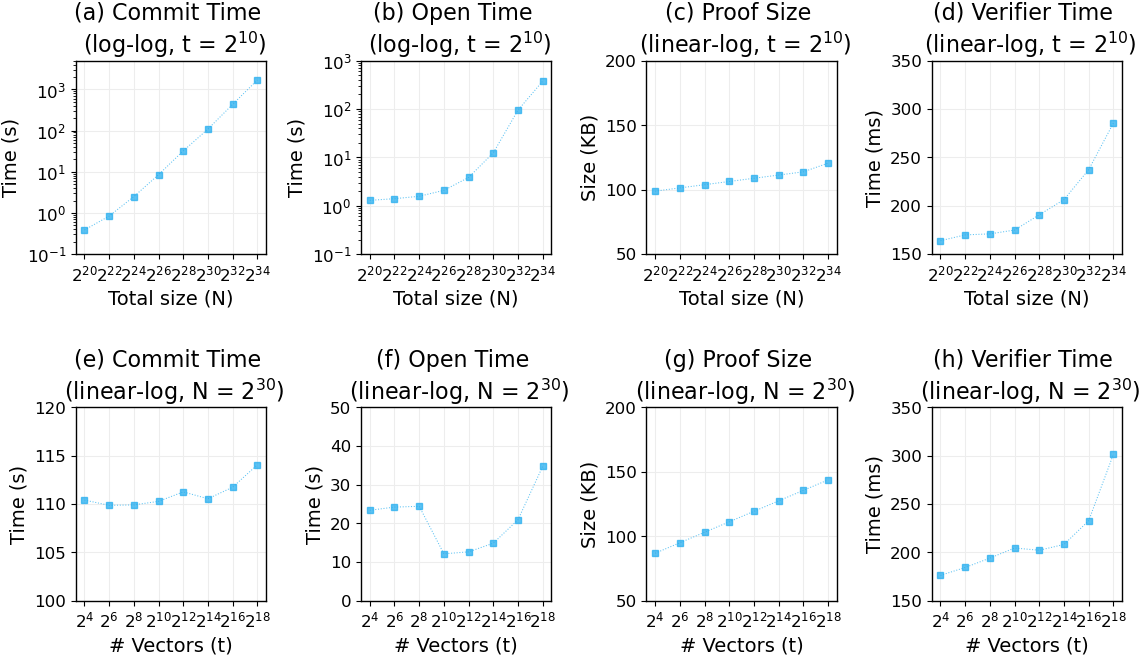
\includegraphics[width=\linewidth]{figure/experiment.png}
\caption{
Performance under
(i) varying total size $N$ with fixed vector count $T$, and
(ii) varying $T$ with fixed total size $N$.
} 
\Description{Experimental results.}
\label{fig:experiment}
\end{figure}


\section{Limitations}
The construction targets the representation boundary between a heterogeneous
vector collection and a multilinear PCS.  Its end-to-end benefit therefore depends on
the fraction of an application's cost attributable to collection commitment
and opening.  Our evaluation isolates this boundary; it does not compare whole
zkML or zkVM proof stacks, whose circuits, claim-reduction protocols, and base
PCS choices differ.  The proven packing bound is $K<4N$, not an optimality
result for all aligned layouts.  Finally, zero materialized-padding overhead
and the stated packing-layer RAM bound require bucket-wise commitment and
low-to-high folding; a base PCS that insists on dense length-$K$ witness
materialization would not preserve these memory properties.
For short-bit-width inputs, the memory advantage assumes native compact storage
and a packed factor $\kappa$ chosen near the field-word-to-input-width ratio;
the packed round adds $2\kappa-2$ field elements to the proof and its polynomial
products cost $O((N/\kappa)M(\kappa))$.  The reported experiments exercise
native 8-bit storage and bucket-wise conversion, but do not separately isolate
the speedup or memory reduction of the packed first round.  Model-parameter
privacy additionally relies on the hiding base commitment and zero-knowledge
composition; the collection layout intentionally reveals public cover buckets.
The size-private mode hides exact dimensions only within the declared leakage
profile: it reveals $T$, $K$, each power-of-two cover $q_j$, and their order, and
an application circuit can reveal dimensions independently.  Its one-time
size-consistency proof is not included in the reported measurements.

\section{Conclusion}
ParComm makes the physical cost of committing a private, quantized model track
its parameters rather than representation expansion.  BVA places the
vectors in a decreasing-size, aligned domain of length $K<4N$ but stores only
the $N$ input entries and compact layout metadata.  TBV provides the matching
compact query representation.  Packed EO-LiteBullet consumes consecutive
stride-$\kappa$ short-input segments and materializes only the reduced field
state.  Together, these mechanisms allocate neither length-padding coordinates
nor an $N$-element field-width expansion, and introduce no packing-layer
auxiliary-RAM term proportional to $K$.
The size-private collection object additionally binds exact matrix dimensions
behind a hiding commitment and a cached consistency proof, so repeated openings
reveal only the public cover layout.

With a bucket-wise linear-prover multilinear PCS, collection commitment and
opening each take $\Theta(N+T\log N)$ prover time for fixed $\kappa$.  Native
$b$-bit inputs use only $O(N/\kappa+T\log N)$ field-valued working
state, with no term proportional to $K$; proof size and verifier time remain
$\Theta(\log N)$.  At $2^{34}$-entry
scale, our heterogeneous instance has a $2^{35}$-coordinate logical domain but
does not allocate its padded coordinates.  The implementation commits in
$29.4$ minutes, opens in $6.4$ minutes, produces a $103$\,KB proof verified in
$0.33$ seconds, and peaks at $404$\,GB of RAM.  Compact collection commitment
therefore remains practical even when a dense representation of the logical
domain would exceed the available memory.


%-------------------------------------------------------------------------------
% Required/recommended USENIX appendices appear immediately after the body.
\cleardoublepage
\appendix
% !TEX root = main.tex
\section*{Ethical Considerations}
\label{app:ethics}
This work studies cryptographic protocols using generated benchmark matrices.
It involves no human participants, personal or sensitive data, proprietary
datasets, deployed systems, or third-party data collection, and therefore
introduces no participant or data-collection risks.

% !TEX root = main.tex
\section*{Open Science}
\label{app:open-science}
Our anonymous artifact at
\url{https://anonymous.4open.science/r/batch-0311} contains the \methodname
implementation, benchmark and plotting scripts, and logs needed to reproduce
our results.

\section{Background}
\label{appx:background}

\subsection{Deferred Definitions}
\label{appx:definitions}
An argument of knowledge allows a computationally bounded prover $\Prover$ to convince a verifier $\Verifier$ that he knows a witness $w$ for a statement~$u$.
\begin{definition}[Argument of Knowledge]
	\label{def: argumentOfKnowledge}
	%The triple
	$(\Setup, \Prover, \Verifier)$ is called an argument of knowledge for the relation $\Relation$ if it satisfies perfect completeness and computational knowledge soundness.
	%as defined below.
\end{definition}

% \cite{groth16_groth2016size}
\begin{definition}[Perfect Completeness]
	\label{def: completeness}
	$(\Setup, \Prover, \Verifier)$ has perfect completeness if for any non-uniform PPT adversary $\Adversary$:
	\begin{equation*}
		% \label{eq:completenessDef}
		\Pr
		\left(
			\left.
				\begin{aligned}
					& (\srs, u, w) \notin \Relation \quad \vee \\
					& \Verifier(\srs, u; \pi) = \TRUE \\
				\end{aligned}
			\right.
			\left |
				\begin{aligned}
					& \srs \leftarrow \Setup(1^{\lambda}); \\
					& (u, w) \leftarrow \Adversary(\srs);\\
					& \pi \leftarrow \PVinteract(\srs, u: w)
				\end{aligned}
			\right.
		\right)
		= 1,
	\end{equation*}
	where $\srs, u, w$, and $\pi$ stand for the structured reference string, the statement, the witness, and the transcript, respectively.
\end{definition}

\begin{definition}[Soundness~\cite{iacr/CanettiCHLRR18}]
	\label{def:soundness}
	$(\Setup, \Prover, \Verifier)$ for a relation $\mathcal{R}$ has a soundness error $\kappa^\mathsf{s}(u)\colon \mathbb{N} \mapsto [0, 1]$ if for any unbounded interactive $\Prover^*$, the probability 
	below
	%that $\Prover^*$ outputs an accepting transcript 
	is bounded by $\kappa^\mathsf{s}(u)$.
	If $\kappa^\mathsf{s}(u)$ is negligible,
	the protocol is sound.
	\begin{equation*}
	% \label{eq:soundnessExpectedTime}
	\Pr
		\left(
			\left.
			\begin{aligned}
				& \Verifier(\pp, u, \pi) = \TRUE \\
			\end{aligned}
			\right.
			\left|
			\begin{aligned}
				& u \notin \Relation;~ \pi \leftarrow (\Prover^* \interact \Verifier) (\pp, u) \\
			\end{aligned}
			\right.
		\right)
	\le \kappa^\mathsf{s}(u).
	\end{equation*}
\end{definition}

\begin{definition}[Knowledge Soundness~\cite{crypto/AttemaCK21}]
	\label{def: soundnessExtract}
	%\quad
	%\phantom{}\\
	$(\Setup, \Prover, \Verifier)$ for relation $\Relation$ is knowledge sound with error $\kappa_{\lambda}(|u|) \colon \mathbb{N} \rightarrow [0, 1]$ if there exists an algorithm $\Extractor$, called a knowledge extractor, given a statement $u$ and black-box oracle access to a (potentially dishonest) prover $\Prover^*$, 
		%the extractor $\Extractor$ 
		it runs in an expected number of steps polynomial in $|u|$ (counting queries to $\Prover$ as a single step) and outputs a witness $ (\srs, u: w) \in \Relation$ with probability: 
	%\begin{equation*}
		% \label{eq:soundnessExpectedTime}
		\[
		\Pr((\srs, u \colon \Extractor(u) ) \in \Relation) 
		\ge
		\frac
		{p(\Prover^*, u) - \kappa_{\lambda}(|u|)}
		{\Poly(|u|)},
		\]
	%\end{equation*}
	where $p(\Prover^*, u)$ is the probability that $\Prover^*$ generates 
	%an accepted
	a valid proof.
\end{definition}



\begin{definition}[Public-Coin]
	\label{def: publicCoin}
	A $(2 \mu + 1)-$move public-coin interactive protocol $(\Setup, \Prover, \Verifier)$ is public-coin if in the $(2j)$-th move, $\Verifier$ sends the $j$-th challenge $x_j \ChooseRandom \mathbb{X}_j$.
	All challenges $x_1, \ldots, x_{\mu}$ sent from the verifier to the prover are public information and chosen uniformly at random and independently of the prover's messages.
\end{definition}

\begin{definition}[Adaptive Fiat-Shamir Transformation]
	The adaptive Fiat-Shamir transformation on a $(2\mu + 1)-$move public-coin interactive protocol: $\mathsf{FS}(\Setup, \Prover, \Verifier) \mapsto (\Setup, \Prover_\mathsf{FS}, \Verifier_{\mathsf{FS}})$ is a two-round argument of knowledge where $\Prover_\mathsf{FS}(\srs, u, w)$ runs $\Prover(\srs, u, w)$ but instead of asking the verifier for the challenge $x_i$ on message $a_i$, the challenges are computed as: 
	\begin{equation*}
		% \label{eq:fiatShamirTransform}
		x_j = \mathsf{Hash}_i(u, a_1, \ldots, a_{j - 1}), \quad j \in [\mu].
	\end{equation*}
the output is then the transcript $\pi = (a_1, \ldots, a_{\mu - 1}, a_{\mu})$.
On input of a statement $u$ and a transcript $\pi = (a_1, \ldots, a_{\mu -1 }, a_{\mu}) $, $\Verifier_{\mathsf{FS}}(\srs, u, \pi)$ accepts if, for $x_j, j \in [\mu]$ as above, $\Verifier$ accepts the transcript $\pi = (a_1, \ldots, a_{\mu - 1}, a_{\mu})$ on input $u$.
\end{definition}


\begin{definition}[Perfect Zero-Knowledge]
\label{def: perfectZeroKnowledge}
	A non-interactive argument of knowledge $(\Setup, \Prover, \Verifier)$ is perfect zero-knowledge~\cite{eurocrypt/Groth16} if there exists a PPT simulator $\Simulator$ and a trapdoor $\mathsf{trap}$ such that for all stateful distinguishers $\Distinguisher$ the following two probabilities are equal:
	\begin{equation*}
		% \label{eq:perfectZeroKnowledge}
		\left.
			\begin{aligned}
			&
			\Pr
			\left(
				\left.
					\begin{aligned}
						& \Distinguisher(\srs, u; \pi; \mathsf{trap}) = \TRUE 
					\end{aligned}
				\right.
				\left |
					\begin{aligned}
						& (\srs, \mathsf{trap}) \leftarrow \Setup(1^{\lambda}); \\
						& \pi \leftarrow \PVinteract (\srs, u: w)
					\end{aligned}
				\right)
			\right.
			\\
			= & 
			\Pr
			\left(
				\left.
					\begin{aligned}
						& \Distinguisher( \srs, u; \pi^*; \mathsf{trap}) = \TRUE \\
					\end{aligned}
				\right.
				\left |
					\begin{aligned}
						& (\srs, \mathsf{trap}) \leftarrow \Setup(1^{\lambda}); \\
						& \pi^* \leftarrow \Simulator (\srs, u; \mathsf{trap})
					\end{aligned}
				\right.
			\right).
			\end{aligned}
		\right.
	\end{equation*}
\end{definition}

\begin{definition}[zkSNARK]
	\label{def:succinctness}
	A zero-knowledge non-interactive argument of knowledge $(\Setup$, $\Prover$, $\Verifier)$ is a succinct non-interactive argument of knowledge (zkSNARK) if:
	\begin{itemize}
	\item The setup time is quasilinear in witness size;
	\item The prover time is quasilinear in witness size;
	\item The proof size is polylogarithmic in witness size;
	\item The verifier time is polylogarithmic in witness size.
	\end{itemize}
\end{definition}



\subsection{Lookup Proof}
\label{appx:lookup}
Lookup proofs allow a prover to show that a collection of queried values,
such as the entries of a matrix $\bm{A}$, are contained in a prescribed
table $\bm{t}\in\Field^m$.
They are a useful primitive in many proof systems:
\eg, they support sparse matrix arithmetization as in
Spartan~\cite{crypto/Setty20}, memory and address consistency in zkVM systems
such as Jolt~\cite{eurocrypt/ArunST24}, and the verification of nonlinear
functions in zero-knowledge machine learning~\cite{ccs/SunLZ24}. Motivated by
these applications, many efficient lookup arguments have been proposed,
including log-derivative lookup (LogUp)~\cite{iacr/Habock22a}, Lasso~\cite{eurocrypt/SettyTW24}, and
Twist and Shout~\cite{iacr/SettyT25}.
We choose LogUp because it scales well for large lookup instances.

\begin{lemma}[Log-Derivative Lookup~{\cite{iacr/Habock22a}}]
\label{lemma:lookup}
Let $\bm{a} \in \Field^N$ and let $\bm{t} \in \Field^m$ be a lookup table. Then $\{a_i\}_{i=1}^N \subseteq \{t_j\}_{j=1}^m$ as multisets iff there exists a multiplicity vector $\bm{\nu} \in \Field^m$ (with $\nu_j$ counting the occurrences of $t_j$ in $\bm{a}$) such that the rational-function identity:
\[
    \sum_{i=1}^N \frac{1}{x + a_i}
    \;=\;
    \sum_{j=1}^m \frac{\nu_j}{x + t_j},
\]
holds in $\Field(x)$. By the Schwartz--Zippel--DeMillo--Lipton lemma, evaluating both sides at a uniformly random $z \sample \Field$ verifies the identity except with probability at most $(N + m)/|\Field|$.
\end{lemma}

\begin{corollary}
Let $\bm{E} \in \Field^{n\times k}$ be a matrix, let
$\bm{t} \in \Field^m$ be a lookup table, and let
$\bm{J} \in [m]^{n\times k}$ be an index matrix.
Let $\bm{m}=(0,1,\ldots,m-1)^\top$.  If $\bm{E}$ is looked up from
$\bm{t}$ at the positions specified by $\bm{J}$, then there exists
$\bm{\nu} \in \Field^m$ such that, for all $\eta,z\in\Field$ for which the
denominators are nonzero:
\[
    \left\langle
    \frac{\bm{1}}{\bm{1}-z(\bm{E}+\eta\bm{J})},
    \bm{1}
    \right\rangle
    =
    \left\langle
    \frac{\bm{1}}{\bm{1}-z(\bm{t}+\eta\bm{m})},
    \bm{\nu}
    \right\rangle,
\]
where division is entrywise. Conversely, if the indexed lookup relation is
false and independent $\eta,z\sample\Field$ are sampled after $\bm E$ is
fixed, the identity holds with probability at most
$O((nk+m)/|\Field|)$.
\end{corollary}

\begin{proof}
The matrix $\bm{E}$ is looked up from $\bm{t}$ at the positions specified by
$\bm{J}$ exactly when every value-index pair $(E_{i,\beta},J_{i,\beta})$ belongs
to the table of pairs $\{(t_j,j)\}_{j=1}^m$, with multiplicities recorded by
$\bm{\nu}$.  The challenge $\eta$ compresses these pairs as:
\[
    E_{i,\beta} + \eta J_{i,\beta}
    \qquad\text{and}\qquad
    t_j + \eta j.
\]
If the pair multisets differ, equality of the compressed multisets is a
nonzero polynomial condition in $\eta$ of degree at most $nk$.  Except with
probability $O(nk/|\Field|)$, the compressed multisets therefore still differ.
Conditioned on this event, Lemma~\ref{lemma:lookup}, evaluated independently at
$z$, accepts with probability at most $(nk+m)/|\Field|$.  The union bound gives
the stated error.
\end{proof}


\cleardoublepage
% !TEX root = main.tex
\section{Efficient TBV Evaluation}
\label{sec:tbveval}

TBVs can be evaluated directly from their compact descriptions rather than
their expanded length-$K$ representations.  For
$\bm{\zeta}\in\Field^K$, define
\[
\Eval(\bm{\zeta},\bm{y})
:= \langle \bm{\zeta}, \tensorspan{\bm{y}} \rangle
\]
and compute it in time proportional to the TBV description size.

As a warm up, if $\bm{\zeta}=\eta\cdot\tensorspan{\bm{z}}$ with
$\bm{z}\in\Field^{\log_2 K}$ and $\eta\in\Field$, then by the mixed-product property:
\[
\Eval(\bm{\zeta},\bm{y})
=
\eta\cdot\prod_{i=1}^{\log_2 K}(1+z_i y_i),
\]
which can be computed in $O(\log K)$ time.
This observation naturally generalizes to vectors formed by concatenating such
tensor blocks.  The general principle of leaving tensor-structured vectors
implicit is well established: Twist and Shout tensor-decompose one-hot address
vectors~\cite{iacr/SettyT25}, and recent permutation arguments exploit sparse,
structured indicator polynomials~\cite{iacr/BunzCDC25}.  The definition below
adapts this implicit-tensor principle to an aligned concatenation and equips it
with the evaluation, split, fold, and proof operations needed by our packing
layer.

For a TBV $\bm{\zeta}\in\Field^K$ and
$\bm{y}\in\Field^{\log_2 K}$, Eq.~\eqref{eq:evaluation} gives
\[
\Eval(\bm{\zeta},\bm{y})
=
\langle \bm{\zeta}, \tensorspan{\bm{y}} \rangle .
\]
Let $S:=\sum_{i=1}^T k_i$ and $\bm{\xi}:=\tensorspan{\bm{y}}$, and mask its
final suffix according to the layout:
\[
  \bm\xi_{\mathcal L}:=(\xi_0,\ldots,\xi_{S-1})\|\bm{0}^{K-S}.
\]
Because $\bm\zeta$ is zero on the same suffix,
$\langle\bm\zeta,\bm\xi\rangle
=\langle\bm\zeta,\bm\xi_{\mathcal L}\rangle$.
Given the bucket sizes $\{k_i\}_{i\in[T]}$, the masked vector
$\bm\xi_{\mathcal L}$ admits a TBV representation with the same bucket
structure:
\[
\bm{\xi}_{\mathcal L}
=
\big(K,T,\{(k_i,\eta_i',\bm{z}_i')\}_{i\in[T]}\big),
\]
where:
\[
\eta_i'
=
\xi_{K_{i-1}}
=
\prod_{q=\log_2 k_i+1}^{\log_2 K}
\bigl(1-\iota_{i,q}+\iota_{i,q}y_q\bigr),
\qquad
\bm{z}_i'=\bm{y}_{[1:\log_2 k_i]},
\]
and $\iota_{i,q}$ denotes the $q$-th least-significant bit of $K_{i-1}$.
Note that, since $k_i$ divides $K_{i-1}$, the first $\log_2 k_i$ entries of the
little-endian binary representation of $K_{i-1}$ are zero.
By Property~\ref{prop:iptbv}, we obtain:
\begin{equation}
\label{eq:tbveval}
\Eval(\bm{\zeta},\bm{y})
=
\sum_{i=1}^T
\eta_i
\cdot
\prod_{q=\log_2 k_i+1}^{\log_2 K}
\bigl(1-\iota_{i,q}+\iota_{i,q}y_q\bigr)
\cdot
\prod_{q=1}^{\log_2 k_i}(1+z_{i,q}y_q),
\end{equation}
which can be evaluated in $\Theta(T\log K)$ time.


% Security proofs are collected at the end of the appendices.
\cleardoublepage
% !TEX root = main.tex
\section{Security Proofs}
\label{appx:securityproofs}

\subsection{Packed EO-LiteBullet}
\label{appx:proof-packed-eo-litebullet}

\begin{proof}[Proof of Theorem~\ref{thm:packedeolitebullet}]
Perfect completeness follows from Eqs.~\eqref{eq:packed-eo-claim}
and~\eqref{eq:binary-eo-fold}.  For soundness of the packed round, let
$\widehat c_h$ denote the coefficient sent for exponent $h\ne0$ by a
potentially dishonest prover.  If the claimed inner product is false, then
\[
  X^{\kappa-1}\left(
    \langle\bm g_a(X),\bm g_b(X)\rangle-c
    -\sum_{h=1}^{\kappa-1}
      (\widehat c_hX^h+\widehat c_{-h}X^{-h})
  \right)
\]
is a nonzero polynomial of degree at most $2\kappa-2$.  It vanishes at a
uniformly sampled $y_0\in\Field^*$ with probability at most
$(2\kappa-2)/(p-1)$.

After bit reversal, each remaining EO round is a LiteBullet round and
contributes soundness error at most $2/(p-1)$.  A union bound over the
$\log_2(K/\kappa)$ binary rounds gives the claimed soundness error.  The proof
contains $2\kappa-2$ packed-round coefficients, two cross terms per binary
round, and the final two scalars.
\end{proof}

\subsection{ParComm}
\label{appx:proof-parcomm}

\begin{proof}[Proof of Theorem~\ref{thm:parcomm-security}]
For completeness, Eq.~\eqref{eq:bva-tbv-batch} rewrites the random linear
combination of valid claims as the BVA--TBV inner product.  Packed
EO-LiteBullet then produces the two valid reduced claims in
Eq.~\eqref{eq:parcomm-reduced-claims}.  The Dory openings accept the claims on
$\bm a$ and $\bm v$, and the TBV evaluation proof accepts the claim on
$\bm\zeta$.  The size-consistency proof accepts witnesses satisfying
Eq.~\eqref{eq:size-private}.  Hence an honest execution is accepted.

For soundness, binding of $C_a$, $C_I$, $C_V$, and $C_X$ fixes the BVA, its
layout, the claimed values, and the evaluation points.  Suppose that at least
one equation in Eq.~\eqref{eq:individual-evaluations} is false, and define
\[
  R(X):=\sum_{j\in[T]}X^{j-1}
  \left(v_j-\tensorproj{\bm a_j}{\bm x_j}\right).
\]
Then $R$ is a nonzero polynomial of degree at most $T-1$.  Consequently,
$R(\omega)=0$ for uniformly sampled $\omega\in\Field^*$ with probability at
most $(T-1)/(p-1)$.  Outside this event, the value bound to $C_V$ cannot satisfy
both Eq.~\eqref{eq:batcheval} and the inner-product claim in
Eq.~\eqref{eq:bva-tbv-batch}.

Theorem~\ref{thm:packedeolitebullet} bounds the probability that an invalid
inner-product claim reaches accepting reduced claims by
\[
  \frac{2\kappa-2+2\log_2(K/\kappa)}{p-1}.
\]
Conditioned on both algebraic checks succeeding, the Dory openings bind
$\bar a$ to the original BVA and $c$ to $\bm v$, while the TBV evaluation proof
binds $\bar b$ to the TBV determined by $\bm I$ and $\bm Z$.  Their remaining
aggregate errors are, by assumption,
$\epsilon_{\mathsf{Dory}}+\epsilon_{\mathsf{tbv}}$.  Finally,
$\pi_{\mathsf{size}}$ binds the private dimensions and effective lengths to
$C_a$ and the public covers except with probability
$\epsilon_{\mathsf{size}}$.  A union bound gives the stated error.
\end{proof}

\subsection{Dimension Privacy}
\label{appx:proof-size-privacy}

\begin{proof}[Proof of Proposition~\ref{prop:size-privacy}]
Consider two valid collections with the same public cover profile
$(T,\{q_j\},\mathcal L)$ and the same public opening statements.  By commitment
hiding, the commitments $C_D$ and $C_a$ for the first collection are
computationally indistinguishable from the corresponding commitments for the
second collection.  Zero knowledge replaces the size-consistency proof and all
opening proofs by simulated transcripts for their fixed public statements.
The remaining public objects, including $C_I$, are deterministic functions of
the shared cover layout.  The verifier's two views are therefore
computationally indistinguishable, so the view reveals no additional
information about $\{r_j,c_j,n_j\}$.
\end{proof}

\subsection{TBV Grand Product}
\label{appx:proof-grand-product}

\begin{proof}[Proof of Lemma~\ref{lem:tbv-grand-product}]
Expanding the first equality gives
\begin{equation}
\label{eq:grandprodproof1}
  w_1+w_2\theta+\cdots+w_m\theta^{m-1}-1
  =\theta\left(w_1'+w_2'\theta+\cdots+w_{m-1}'\theta^{m-2}\right).
\end{equation}
The equality $\bm w'=\bm a\circ\bm w$ gives
\begin{equation}
\label{eq:grandprodproof2}
  w_1'=a_1w_1,\quad w_2'=a_2w_2,\quad\ldots,\quad w_m'=a_mw_m,
\end{equation}
and the final constraint gives $c=w_m'$.  Comparing the coefficients of
Eq.~\eqref{eq:grandprodproof1}, except with the Schwartz--Zippel error for the
random $\theta$, yields
\[
  w_1=1,\qquad
  w_2=a_1w_1,\quad
  w_3=a_2w_2,\quad\ldots,\quad
  w_m=a_{m-1}w_{m-1}.
\]
Thus $w_m=\prod_{i=1}^{m-1}a_i$, and
\[
  c=w_m'=a_mw_m=\prod_{i=1}^m a_i.
\]
\end{proof}


\cleardoublepage
\bibliographystyle{plainurl}
\bibliography{ref}

%%%%%%%%%%%%%%%%%%%%%%%%%%%%%%%%%%%%%%%%%%%%%%%%%%%%%%%%%%%%%%%%%%%%%%%%%%%%%%%%
\end{document}
%%%%%%%%%%%%%%%%%%%%%%%%%%%%%%%%%%%%%%%%%%%%%%%%%%%%%%%%%%%%%%%%%%%%%%%%%%%%%%%%
